% Options for packages loaded elsewhere
\PassOptionsToPackage{unicode}{hyperref}
\PassOptionsToPackage{hyphens}{url}
\documentclass[
]{article}
\usepackage{xcolor}
\usepackage{amsmath,amssymb}
\setcounter{secnumdepth}{5}
\usepackage{iftex}
\ifPDFTeX
  \usepackage[T1]{fontenc}
  \usepackage[utf8]{inputenc}
  \usepackage{textcomp} % provide euro and other symbols
\else % if luatex or xetex
  \usepackage{unicode-math} % this also loads fontspec
  \defaultfontfeatures{Scale=MatchLowercase}
  \defaultfontfeatures[\rmfamily]{Ligatures=TeX,Scale=1}
\fi
% \usepackage{lmodern}
\ifPDFTeX\else
  % xetex/luatex font selection
\fi
% Use upquote if available, for straight quotes in verbatim environments
\IfFileExists{upquote.sty}{\usepackage{upquote}}{}
\IfFileExists{microtype.sty}{% use microtype if available
  \usepackage[]{microtype}
  \UseMicrotypeSet[protrusion]{basicmath} % disable protrusion for tt fonts
}{}
\makeatletter
\@ifundefined{KOMAClassName}{% if non-KOMA class
  \IfFileExists{parskip.sty}{%
    \usepackage{parskip}
  }{% else
    \setlength{\parindent}{0pt}
    \setlength{\parskip}{6pt plus 2pt minus 1pt}}
}{% if KOMA class
  \KOMAoptions{parskip=half}}
\makeatother
\usepackage{longtable,booktabs,array}
\newcounter{none} % for unnumbered tables
\usepackage{calc} % for calculating minipage widths
% Correct order of tables after \paragraph or \subparagraph
\usepackage{etoolbox}
\makeatletter
\patchcmd\longtable{\par}{\if@noskipsec\mbox{}\fi\par}{}{}
\makeatother
% Allow footnotes in longtable head/foot
\IfFileExists{footnotehyper.sty}{\usepackage{footnotehyper}}{\usepackage{footnote}}
\makesavenoteenv{longtable}
\usepackage{graphicx}
\makeatletter
\newsavebox\pandoc@box
\newcommand*\pandocbounded[1]{% scales image to fit in text height/width
  \sbox\pandoc@box{#1}%
  \Gscale@div\@tempa{\textheight}{\dimexpr\ht\pandoc@box+\dp\pandoc@box\relax}%
  \Gscale@div\@tempb{\linewidth}{\wd\pandoc@box}%
  \ifdim\@tempb\p@<\@tempa\p@\let\@tempa\@tempb\fi% select the smaller of both
  \ifdim\@tempa\p@<\p@\scalebox{\@tempa}{\usebox\pandoc@box}%
  \else\usebox{\pandoc@box}%
  \fi%
}
% Set default figure placement to htbp
\def\fps@figure{htbp}
\makeatother
\setlength{\emergencystretch}{3em} % prevent overfull lines
\providecommand{\tightlist}{%
  \setlength{\itemsep}{0pt}\setlength{\parskip}{0pt}}
\usepackage[]{natbib}
\bibliographystyle{plainnat}
\usepackage{bookmark}
\IfFileExists{xurl.sty}{\usepackage{xurl}}{} % add URL line breaks if available
\urlstyle{same}
\hypersetup{
  hidelinks,
  pdfcreator={LaTeX via pandoc}}

\author{}
\date{}

\title{The Golden Compass and the Lunar Flux\\\normalsize William Blake, Bimetallic Meta-stability, and the Architecture of Value}
\author{Daniel Ari Friedman\\\footnotesize{Active Inference Institute}\\\footnotesize{\texttt{daniel@activeinference.institute}}\\\footnotesize{\href{https://orcid.org/0000-0001-6232-9096}{ORCID: 0000-0001-6232-9096}} \\ \footnotesize{\href{https://doi.org/10.5281/zenodo.19335196}{DOI: 10.5281/zenodo.19335196}}}
\date{\today}

\usepackage{graphicx}

\makeatletter
\AtBeginDocument{\immediate\write\@auxout{\string\bibdata{references}}}
\makeatother
\begin{document}

\maketitle
\thispagestyle{empty}
\tableofcontents
\newpage


\section{Abstract}\label{abstract}

This manuscript maps the structural collapse of British bimetallism
(1717--1844) onto the mythopoetic architecture of William Blake's
prophetic epics, arguing the disintegration of the gold-silver standard
materially enacted the cosmological fracture Blake dramatized. The
architecture of this entropy formalized on 21 September 1717, when Isaac
Newton, Master of the Royal Mint, established the guinea at 21 silver
shillings---a ratio of 15.21:1 that structurally overvalued gold against
continental markets. Under Gresham's Law, this metric disparity drove
English silver to France and the Far East, hollowed out the domestic
currency, and set the stage for the Bank Restriction crisis of February
1797. When the Bank of England's physical gold reserves collapsed
against a ten-fold circulation of paper notes, the British economy
underwent a systemic \emph{clinamen}---a swerve into the flux of fiat
abstraction. This groundlessness, extensively debated during the
Bullionist Controversy, culminated in the 1816 Coinage Act's statutory
establishment of the gold sovereign and the 1844 Bank Charter Act's
enclosure of value within the ledger. We trace this entropic trajectory
across the Atlantic to the American ``Crime of 1873'' and the 1896
``Cross of Gold'' crusade, revealing a transatlantic monetary framework
Blake first diagnosed in \emph{America A Prophecy}.

To counter this macro-economic atomization, Blake developed his
artisanal \emph{Fourfold Vision} as a systematic epistemology designed
to rescue human valuation from the mechanistic paradigms of capitalist
quantification. Blake's lifelong opposition to Newtonian ``Single
Vision'' aligns with his structural critique of the reductive logic of
monometallism. Where Newton's Mint fixed value within isolated metallic
quanta, Blake asserted the qualitative depths of imaginative perception.
His explicit marginalia against gold (``a guinea is more beautiful than
the sun'' to a miser), his condemnation of ``allegoric riches,'' and his
defense of Thomas Paine constitute a materialist indictment of the
commodification of human experience. By analyzing the physical Mint
alongside Los's spiritual forges as dual engines of socio-metaphysical
reproduction---the former quantifying labor into universal equivalents,
the latter transmuting material into the ``Human Form Divine'' through
relief-etching---this manuscript repositions Blake as a foundational
critic of financialized alienation. His prophetic stance bridges early
industrial monetary policy with the Marxist critique of commodity
fetishism, anticipating contemporary debates over fiat currencies
unmoored from their human ground.

\newpage

\section{Introduction: The Monetary Divide and the Architecture of
Value}\label{introduction-the-monetary-divide-and-the-architecture-of-value}

The late eighteenth century witnessed a fundamental restructuring of
British metaphysics and global monetary policy. Central to this upheaval
was the imposition of material quantification---an epistemological
framework derided by the poet, printmaker, and visionary William Blake:
``May God us keep / From Single vision \& Newtons sleep'' (Letter to
Thomas Butts, 22 November 1802) \citep{erdman1988complete}.
Concurrently, the British economic architecture was paralyzed by the
meta-stable tension of bimetallism. Gold and silver, theoretically bound
by the statutory fiat established by Isaac Newton on 21 September 1717
\citep{horsefield1960british}, operated not as cooperative halves of a
sovereign currency, but as autonomous vectors driven by international
arbitrage. Every monetary system must answer a foundational question:
\emph{what is the unit of account, and who controls its definition?} The
bimetallic answer---that two distinct physical substances could
simultaneously serve as a unified standard---was an inherent
contradiction, a legislative fiction sustained only so long as the
statutory ratio approximated fluctuating market realities.

\subsection{Gresham's Entropy and the Question of
Value}\label{greshams-entropy-and-the-question-of-value}

This dynamic was the purest manifestation of Gresham's Law, explored
extensively in the subsequent section, the principle first articulated
by Thomas Gresham in 1558: when two metals circulate at a fixed ratio
misaligned with market values, the undervalued metal is melted and
exported while the overvalued metal remains \citep{thornton1802nature}.
In the British context, Newton's domestic ratio of 1:15.21 overvalued
gold against continental market ratios near 1:14.5, ensuring artificial
gold drove out undervalued silver. By 1715, nearly all the silver Newton
recoined during the Great Recoinage (1696--1699) had physically left the
country, shipped to France and the East Indies where its bullion weight
commanded a structural premium
\citep{quinn1996competing, quinn2006bank}. The physical disappearance of
metallic currency set the necessary preconditions for the rise of
abstract financial instruments.

\subsection{Blake's Critique of Atomistic Commerce and Financial
Abstraction}\label{blakes-critique-of-atomistic-commerce-and-financial-abstraction}

Blake's lifelong critique of materialist atomism---the Epicurean
reduction of reality to disconnected, self-moving particles---maps
directly onto this escalating monetary abstraction
\citep{schouten2020epicurean}. While the Bank of England increasingly
relied on fractional reserves, paper issuance, and the arithmetic of
compounding imperial debt, Blake saw the fabric of human existence
divided into disconnected units of negotiable property. In \emph{London}
(Songs of Experience, 1794), the poet hears in ``every voice: in every
ban, / The mind-forg'd manacles'' (Plate 46, lines 7--8; Erdman p.~70)
\citep{erdman1988complete}---the invisible chains that commerce, law,
and state finance forge around the human imagination. As Mary Poovey
observes, the late eighteenth century saw the fundamental displacement
of intrinsic value by relational, speculative paper instruments---a
shift that alienated the laboring subject from their own work
\citep{poovey2008genres}.

Jon Mee notes that Blake's prophetic reaction to this crisis was
grounded in the radicalism of the 1790s, where political dissent fused
with critiques of state-sponsored economic policy
\citep{mee1992dangerous}. Blake's allegiance to this milieu is
documented in his annotations to Bishop Richard Watson's \emph{An
Apology for the Bible} (1798), defending Thomas Paine against
establishment slander: ``To defend the Bible in this year 1798 would
cost a man his life. The Beast \& Whore damn the Bible'' (Erdman p.~616)
\citep{erdman1988complete}. E.P. Thompson extends this analysis, reading
Blake's deliberate imagery as a materialist indictment of the
acquisitive ethic---the systematic division of people and the
enforcement of moral bondage through market relations
\citep{thompson1993witness}. The ``dark Satanic Mills'' of the
\emph{Milton} preface (Erdman p.~95) operate simultaneously as the
literal industrial factories of the emerging capitalist order, and the
institutional ``mills'' of the established church grinding individuals
into doctrinal uniformity. As Joseph Albernaz identifies, measurement
technologies---whether the Newtonian standard of 1717 or the impending
1816 Gold Standard---enforce ``chimeric regimes.'' They attempt to
ground society in finite materiality while obfuscating humanity's shared
groundlessness \citep{albernaz2024common}.

\subsection{The Miser's Guinea and the Urizenic
Inversion}\label{the-misers-guinea-and-the-urizenic-inversion}

This structural alienation extends from the macroeconomic sphere into
individual perception. Blake viewed the financial systems of his day not
merely as flawed economic policies, but as ontological regressions. In
his marginalia to Sir Joshua Reynolds' \emph{Discourses} (c.~1808),
Blake launches an explicit attack on this ideological inversion: ``To
the eyes of a miser a guinea is more beautiful than the sun, and a bag
worn with the use of money has more beautiful proportions than a vine
filled with grapes'' (Erdman p.~635) \citep{blake1808annotations}. The
golden guinea usurps the celestial sun; the dead container replaces the
living vine. This critique sharpens when Blake urgently demands in
\emph{Milton}: ``Leave counting Gold \& diamonds, for Gods eye delights
in thee'' (Plate 26, line 27; Erdman p.~121) \citep{erdman1988complete}.
For Blake, emergent capitalism and its central bankers represented a
conceptual flattening of existence, where the Enlightenment God
functioned as a senior accountant processing ledgers of abstract human
life rather than participating in its divine creation. The entire
structure of bimetallic generation and subsequent monometallic isolation
was a symptom of this Urizenic idolatry.

\subsection{Esoteric Finance and the Historiographic
Framework}\label{esoteric-finance-and-the-historiographic-framework}

This historical backdrop has been documented by monetary historians like
Marc Flandreau and Alexander Del Mar.~As Flandreau argues, bimetallism
was an inherently unstable architecture, requiring a precarious
international equilibrium to prevent the collapse of domestic coinage
\citep{flandreau1996bimetallism}. Del Mar takes this further, viewing
the history of money as a constant struggle between state prerogative
(communal sovereignty) and private financial calculus (the
monopolization of coinage by mercantile elites)
\citep{delmar1895history}. David Erdman, in his foundational
\emph{Blake: Prophet Against Empire} (1954), connects Blake's cosmic
visions directly to political economy, interpreting Urizen as the
``great Work master'' who builds his cosmos through ``slave labor''---a
direct textual indictment of imperial war-financing and the
commodification of human energy \citep{erdman1954prophet}. Blake's
prophetic works can be read as an esoteric articulation of this
struggle, a historically consistent political myth that maps the
spiritual descent into Ulro to the materialist pressures of Bank
Restriction-era credit economies
\citep{ferber2003politics, duty2000sublime}.

\subsection{Manuscript Structure and
Methodology}\label{manuscript-structure-and-methodology}

In this manuscript, we explicitly reconstruct the Newtonian Standard,
the 1797 Bank Restriction Act
\citep{clapham1944bank, fetter1965development}, and the 1816 Coinage Act
\citep{redish1990evolution} not as rote economic touchstones, but as
topological fractures precipitating a systemic regression of the human
spirit. We attend to the \emph{minute particulars} of Blake's
engagement---his specific textual attacks on gold, his metallurgical
imagery, his precise plate compositions---while simultaneously tracing
the \emph{generic} structural logic by which any system of rigid
quantification must ultimately devour the qualitative life it claims to
measure. Blakean prophecy enacts a radical ideological inversion:
destroying the atomistic enclosures of Urizen, rejecting the spectral
flux of bimetallic generation, and laboring intensely at the Forges of
Los to rescue human agency and forge the ultimate ``Human Form Divine''
(detailed further under
\href{04a_illuminated_nonduality.md\#illuminated-nonduality-and-the-fourfold-vision}{Illuminated
Nonduality}).

\begin{figure}
\centering
\pandocbounded{\includegraphics[keepaspectratio,alt={Bimetallic and Prophetic Timeline --- Dual-Axis Chronology of Financial Collapse and Prophetic Ascent (1710--1900). Upper axis (Financial Events): progressive disintegration of the bimetallic synthesis from the 1717 Newtonian Standard (M: 1:15.21) through Hamilton's ratio of 15:1 (1792), the 1797 Bank Restriction, and the 1816 British Coinage Act (m\_S \textbackslash to 0), culminating in the ``Crime of 1873'' and Bryan's ``Cross of Gold'' (1896). Lower axis (Blake's Prophetic Works): Blake's inverse prophetic trajectory surges in metaphysical urgency---from The Book of Thel (1789) through America A Prophecy (1793), Songs of Experience (1794), The Four Zoas (1797--1807), and Jerusalem (1804--1820). Shaded era bands mark the British Bank Restriction Period (1797--1821) and the American Greenback Suspension (1862--1879)---twin clinamina of paper groundlessness on opposite shores of the Atlantic {[}@fetter1965development; @laughlin1898bimetallism{]}.}]{../figures/timeline.png}}
\caption{Bimetallic and Prophetic Timeline --- Dual-Axis Chronology of
Financial Collapse and Prophetic Ascent (1710--1900). Upper axis
(Financial Events): progressive disintegration of the bimetallic
synthesis from the 1717 Newtonian Standard (\(M: 1:15.21\)) through
Hamilton's ratio of 15:1 (1792), the 1797 Bank Restriction, and the 1816
British Coinage Act (\(m_S \to 0\)), culminating in the ``Crime of
1873'' and Bryan's ``Cross of Gold'' (1896). Lower axis (Blake's
Prophetic Works): Blake's inverse prophetic trajectory surges in
metaphysical urgency---from The Book of Thel (1789) through America A
Prophecy (1793), Songs of Experience (1794), The Four Zoas (1797--1807),
and Jerusalem (1804--1820). Shaded era bands mark the British Bank
Restriction Period (1797--1821) and the American Greenback Suspension
(1862--1879)---twin clinamina of paper groundlessness on opposite shores
of the Atlantic
\citep{fetter1965development, laughlin1898bimetallism}.}\label{fig-timeline}
\end{figure}

\newpage

\section{Entropic Architectures of Gold and
Silver}\label{entropic-architectures-of-gold-and-silver}

The architecture of British bimetallic entropy was formally codified on
21 September 1717 by the Master of the Royal Mint, Sir Isaac Newton.
Newton, appointed Warden in 1696 through John Locke and Charles Montagu,
and promoted to Master in 1699, approached the currency crisis---the
continuous outflow of English silver to the East India Company and the
continent---with the same geometric precision he applied to the cosmos
in his \emph{Principia}. In his report ``State of the Gold \& Silver
Coins of the Kingdom,'' Newton executed a bureaucratic fiat: he fixed
the golden guinea at exactly 21 silver shillings, establishing a
domestic gold-to-silver ratio of approximately 1:15.21
\citep{quinn1996competing}.

This valuation led to a Royal Proclamation on 21 December 1717. Newton
claimed to have brought the coinage to ``a much greater degree of
exactness than ever was known before,'' relying on Trial Plates and
mathematical ratios to formally weigh out the realm
\citep{horsefield1960british}. For William Blake, however, this
exactness was not a stabilizing measure but an ontological constraint.
Newton's intervention epitomizes the Urizenic instinct: the attempt to
arrest the living flux of human exchange by superimposing a geometric
grid.

\subsection{The Alchemy of the Mint and the Geometry of
Death}\label{the-alchemy-of-the-mint-and-the-geometry-of-death}

Newton's role presents a historical paradox that aligns with Blake's
mythological critique. While enforcing the mechanistic ratios of the
1717 standard, Newton was simultaneously immersed in clandestine
alchemical pursuits, experimenting with transmutations and esoteric
theology \citep{schouten2020epicurean}. Yet his public legacy at the
Mint stripped currency of its qualitative, alchemical vitality.

Blake isolates this paradox in his 1795 color print \emph{Newton}. The
scientist sits naked at the bottom of the ocean, his gaze fixed downward
upon a geometric scroll, wielding golden compasses---the exact
instruments of the Mint's standardization. Just as Urizen creates the
material world by division---binding the infinite with the ``golden
compass'' and ``brazen quadrant'' (\emph{The First Book of Urizen})
\citep{blake1795urizen}---Newton's valuation clamped down upon the
living economy. Imposing rigid numerics over the transformative
alchemical process, Newton institutionalized the ``Single Vision'' Blake
fought to break. The print is not merely an aesthetic critique of
empiricism; it is a historically precise indictment of the metrological
regime Newton imposed upon the imperial world
\citep{albernaz2024common, makdisi2003william}.

\subsection{The Structural
Overvaluation}\label{the-structural-overvaluation}

Furthermore, Newton's 1:15.21 domestic ratio structurally overvalued
gold against fluctuating international bullion markets, which hovered
near 1:14.5 in France and 1:15 across Europe \citep{quinn2006bank}. A
guinea worth 21 shillings in England was priced at roughly 20s 9d in
Portugal or France. This mathematical misalignment, rather than
fostering stability, guaranteed that gold---particularly Brazilian gold
via Portugal---flooded English ports, while ``undervalued'' silver was
siphoned abroad. By 1715, nearly all the silver Newton struck during the
Great Recoinage (1696--1699) had vanished to France and the East Indies
\citep{quinn1996competing}. The Bank of England amassed 15.5 tonnes of
gold by 1730 from these asymmetric flows, inadvertently shifting Britain
toward gold dominance.

\begin{figure}
\centering
\pandocbounded{\includegraphics[keepaspectratio,alt={The Arbitrage Fracture --- Transatlantic Divergence of British, American, and Market Ratios (1717--1873). Three lines trace the divergent monetary architectures: Newton's frozen English Mint Ratio (15.21:1, dashed white), Hamilton's US Mint Ratio (15:1 → 16:1 after 1834, green), and the fluctuating European market reality (gold). Key event markers indicate the US Coinage Act (1792), Bank Restriction (1797), British Coinage Act (1816), US ratio revision (1834), and the ``Crime of 1873.'' The shaded regions between Newton's line and the market ratio represent the Gresham ``escape velocity''---the precise profit margin that drove bullion arbitrageurs to drain England's circulating silver. Hamilton's deliberate undervaluation of gold at 15:1 produced the mirror drainage: American gold flowed to Europe, making silver the de facto US standard until the 1834 correction {[}@flandreau1996bimetallism; @laughlin1898bimetallism{]}.}]{../figures/historic_ratio.png}}
\caption{The Arbitrage Fracture --- Transatlantic Divergence of British,
American, and Market Ratios (1717--1873). Three lines trace the
divergent monetary architectures: Newton's frozen English Mint Ratio
(15.21:1, dashed white), Hamilton's US Mint Ratio (15:1 → 16:1 after
1834, green), and the fluctuating European market reality (gold). Key
event markers indicate the US Coinage Act (1792), Bank Restriction
(1797), British Coinage Act (1816), US ratio revision (1834), and the
``Crime of 1873.'' The shaded regions between Newton's line and the
market ratio represent the Gresham ``escape velocity''---the precise
profit margin that drove bullion arbitrageurs to drain England's
circulating silver. Hamilton's deliberate undervaluation of gold at 15:1
produced the mirror drainage: American gold flowed to Europe, making
silver the de facto US standard until the 1834 correction
\citep{flandreau1996bimetallism, laughlin1898bimetallism}.}\label{fig-historic-ratio}
\end{figure}

\subsection{The Triumph of Single
Vision}\label{the-triumph-of-single-vision}

The Newtonian standard did not stabilize value; it maximized the margin
between statutory decree and market reality, fueling the arbitrage it
sought to suppress. It instituted a mechanistic worldview where wealth
derived not from prophetic creation or human labor, but from the
calculation of metallic ratios. This was the triumph of \emph{Single
Vision}---the reduction of qualitative human life to quantitative,
fungible units. The living vine of human interaction was severed,
replaced by the unyielding geometry of the coin. As Northrop Frye
identifies in \emph{Fearful Symmetry}, Blake's opposition to this regime
was a fully articulated philosophical telos: Fourfold Vision as the
restoration of imaginative creativity operating against the ``tyranny of
custom'' and the ``placid ovine herd'' of market-driven uniformity
\citep{frye1947fearful}.

\newpage

\section{Gresham's Law and the Fracture of Esoteric
Alchemy}\label{greshams-law-and-the-fracture-of-esoteric-alchemy}

When international silver values fluctuated against the enforced
Newtonian mint ratio of 1717, they triggered the mechanical arbitrage of
Gresham's Law: ``bad money drives out good'' \citep{thornton1802nature}.
Because gold was systematically overvalued within the English
Channel---Newton's guinea priced at 21 shillings domestically while
equivalent gold commanded only 20s 9d in Spain or Portugal---bullion
merchants melted full-weight silver coins and shipped the raw bullion to
France, India, and China, where its elemental weight commanded
significantly higher purchasing power \citep{quinn1996competing}. An
engineered mathematical disparity hollowed out the domestic money
supply.

\subsection{Velde's Mathematical Formalism of Bimetallic
Instability}\label{veldes-mathematical-formalism-of-bimetallic-instability}

To formalize this entropic decay, modern economic historians such as
François Velde define the bimetallic equilibrium via the relationship
between the statutory Mint Ratio (\(M\)) and the global commodity Market
Ratio (\(R\)), bounded by transaction and melting costs (\(c\))
\citep{velde2005bimetallism}. The condition for a functional,
meta-stable bimetallic circulation is expressed mathematically as:

\begin{equation}
\label{eq:bimetallic_bounds}
M - c < R < M + c
\end{equation}

When the international market ratio of silver to gold climbs beyond the
domestic limit erected by the state (\(R > M + c\)), silver becomes
undervalued at the mint. Arbitrageurs mathematically optimize their
portfolios by melting down full-weight silver coins---the ``Lunar
Flux''---and exporting the bullion to France, India, or the Far East,
where its elemental weight commands a higher purchasing power. The East
India Company played a central role in this drainage, trading English
silver in Asia where it commanded premium value amid regional gold
scarcity; by 1730, these asymmetric flows had delivered 15.5 tonnes of
gold into the Bank of England's vaults while emptying the kingdom of
circulating silver \citep{quinn2006bank}. This arbitrage drained the
physical economy of its circulating medium, leaving behind only clipped,
worn, or counterfeit silver, alongside the static, hoarded gold.

\subsection{Del Mar's Esoteric Reading of the Bimetallic
Marriage}\label{del-mars-esoteric-reading-of-the-bimetallic-marriage}

However, analyzing this financial collapse exclusively through
quantitative arithmetic obscures its ontological
implications---implications that William Blake recognized implicitly.
The 19th-century monetary historian Alexander Del Mar later framed this
dual-standard through an esoteric lens that resonates with Blakean
mythology. In his structural historiographies of money, Del Mar casts
bimetallic equilibrium not merely as an economic truce, but as an
attempt at divine harmonics: a socio-political synthesis where the solar
and lunar metals maintain equilibrium in the monetary firmament under
the sovereign prerogative of the state \citep{delmar1895history}. Del
Mar writes extensively on the sacred, often solar and lunar origins of
coinage in antiquity, viewing the gold-silver pairing as a degraded
remnant of a dualistic religious system representing divine
authority---the alchemical marriage of Sol and Luna that underwrites
legitimate sovereignty. Marc Flandreau extends this historiography,
characterizing classical bimetallism as a form of economic alchemy
conjuring stabilizing stasis from the metaphysical chaos of global trade
by binding two independent metallic volatilities into a single legal
fiction \citep{flandreau1996bimetallism}.

\subsection{The Decay from Generation to
Ulro}\label{the-decay-from-generation-to-ulro}

London's legally entrenched overvaluation of gold severed this
alchemical harmony \citep{quinn1996competing}. Bimetallism was,
inherently, a \emph{Twofold Generative} tension (see the Four Levels of
Vision): an unstable but vitalizing socio-economic synthesis of the
Solar (Gold/Love/Authority) and the Lunar (Silver/Wisdom/Circulation).
The bullion merchants---driven by the atomizing, Epicurean
\emph{clinamen} of profit and private self-interest---melted down the
lunar element to hoard the solar. As David Erdman identifies in
\emph{Blake: Prophet Against Empire}, this rapacity maps directly onto
Blake's depiction of Urizen as the ``great Work master'' who builds his
empire through slave labor and imperial war-financing
\citep{erdman1954prophet}.

For Blake, this is the very definition of the state of \emph{Generation}
decaying into \emph{Ulro} (the void). Production and exchange were no
longer aimed at sustaining human community or fulfilling human needs,
but were captured by the ``spectral flux'' of arbitrage. When Blake
writes in \emph{Jerusalem} that the ``Councellor'' seeks ``To fix the
price of labour; / To invent allegoric riches'' (Plate 27, lines 10--14;
Erdman p.~170) \citep{erdman1988complete, sklar2011blake}, he describes
precisely this structural capture: the moment when the living economy of
human exchange is seized by the arithmetic of financial extraction. The
bimetallic synthesis fractured under the friction of Gresham's entropy,
driving the entire system toward the mathematical void of monometallic
isolation (as detailed in the discussion of the 1816 Coinage Act).
Gresham's law, in this esoteric register, is not merely a law of
economics, but a law of spiritual thermodynamics: the inevitable
degradation of meaning when human relationships are mediated exclusively
by rigid metrics.

\begin{figure}
\centering
\pandocbounded{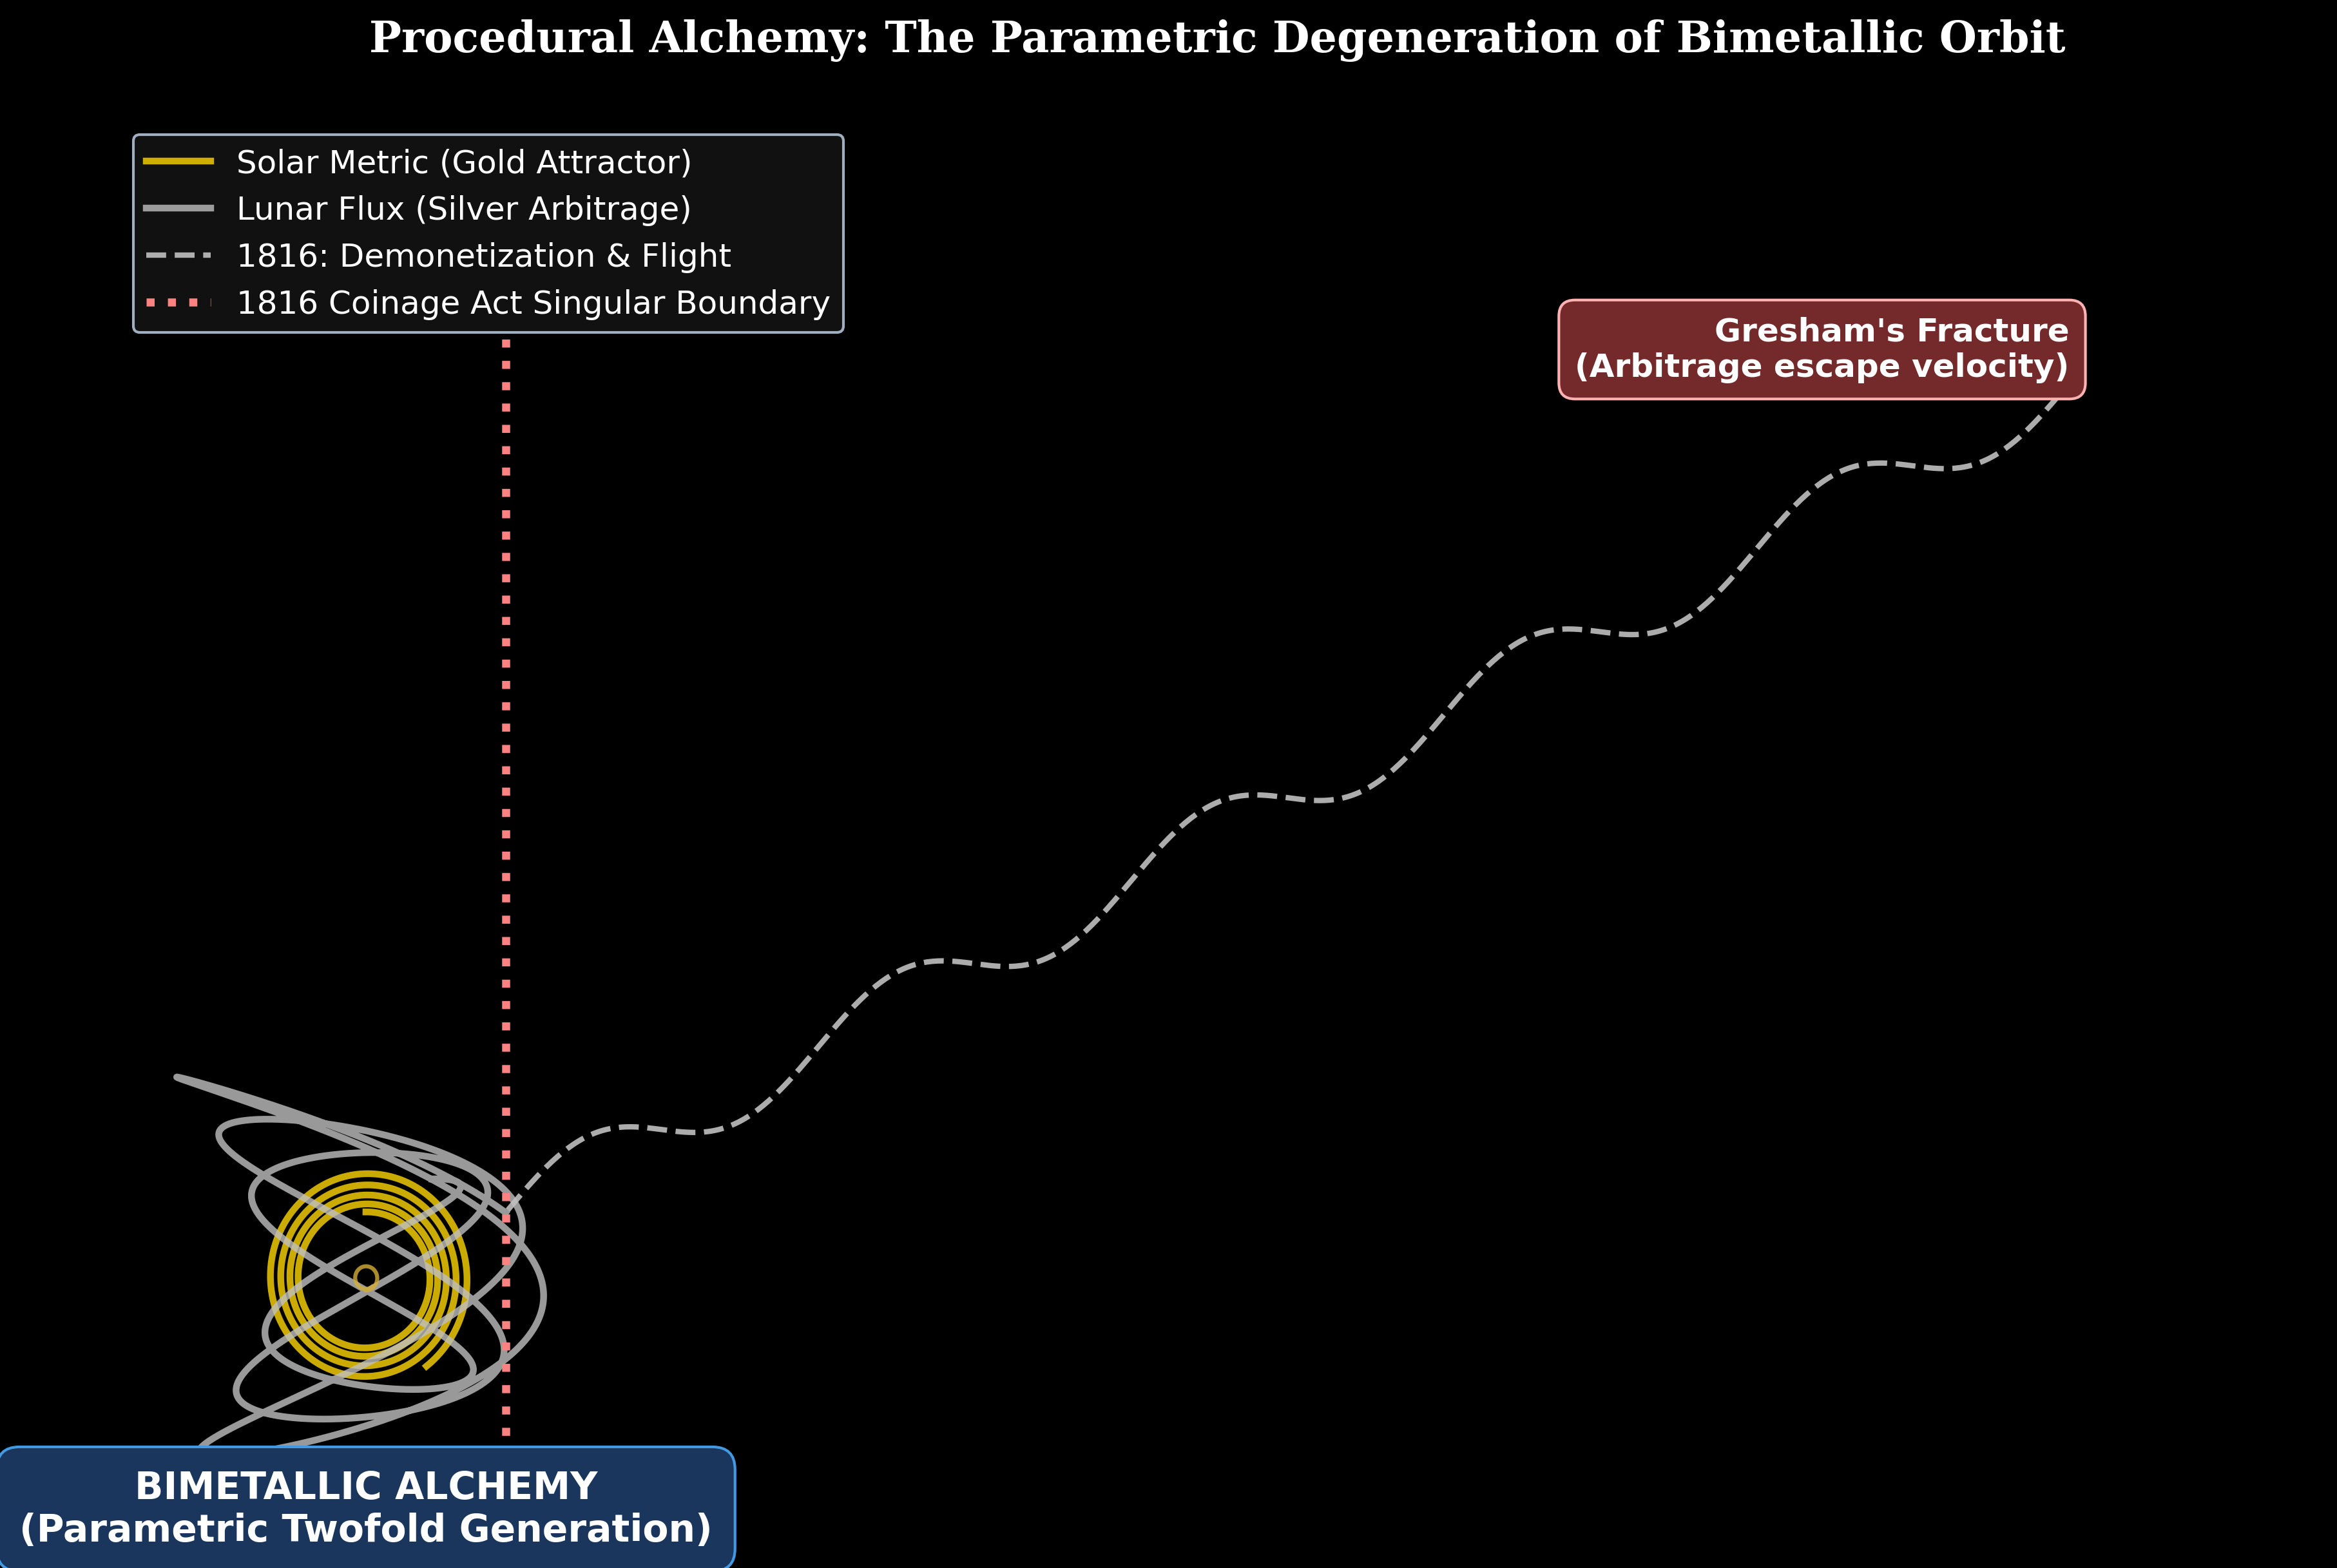
\includegraphics[keepaspectratio,alt={Procedural Alchemy of Bimetallic Vectors --- Parametric Degeneration of Bimetallic Orbit. This procedurally generated Harmonograph maps the historical vectors of Solar Gold (the central, tight attractor) and Lunar Silver (the wider, sweeping orbit of the 1.5 ratio) locked in meta-stable Twofold Generation. Mathematical harmony holds until Velde's bounding thresholds are breached (R \textgreater{} M + c). At the 1816 singular boundary, Gresham's arbitrage escape velocity is crossed: the Solar Gold vector collapses inward to a static geometric dot (Single Vision / The Gold Standard), while the Lunar Silver vector violently breaks orbit, escaping tangentially into chaotic, infinitely speculative space---modeling the physical demonetization of silver under the Coinage Act (56 Geo. III c.68) and the total eradication of the bimetallic generative synthesis.}]{../figures/alchemical_bimetallism.png}}
\caption{Procedural Alchemy of Bimetallic Vectors --- Parametric
Degeneration of Bimetallic Orbit. This procedurally generated
Harmonograph maps the historical vectors of Solar Gold (the central,
tight attractor) and Lunar Silver (the wider, sweeping orbit of the 1.5
ratio) locked in meta-stable Twofold Generation. Mathematical harmony
holds until Velde's bounding thresholds are breached (\(R > M + c\)). At
the 1816 singular boundary, Gresham's arbitrage escape velocity is
crossed: the Solar Gold vector collapses inward to a static geometric
dot (Single Vision / The Gold Standard), while the Lunar Silver vector
violently breaks orbit, escaping tangentially into chaotic, infinitely
speculative space---modeling the physical demonetization of silver under
the Coinage Act (56 Geo. III c.68) and the total eradication of the
bimetallic generative synthesis.}\label{fig-alchemy}
\end{figure}

\newpage

\section{The 1797 Bank Restriction and the Suspension of Metallic
Reality}\label{the-1797-bank-restriction-and-the-suspension-of-metallic-reality}

The meta-stable tension of Twofold bimetallism finally shattered under
the structural geopolitical pressures of the French Revolutionary Wars.
By the late 1790s, Britain was facing a multidimensional crisis of
liquidity, sovereignty, and national survival. Panic swept the
countryside as rumors of French invasion---dramatically realized by the
Battle of Fishguard (22--24 February 1797), the last foreign invasion
force to land on British soil---prompted local farmers and mercantilists
to storm the provincial banks, demanding hard gold for their paper
notes. These localized runs cascaded into Threadneedle Street.

\subsection{The Collapse of Reserves and the Privy Council
Order}\label{the-collapse-of-reserves-and-the-privy-council-order}

By the end of February 1797, the Bank of England's gold reserves had
dwindled to critical levels---just £1,086,170 against total note
circulation of £10,865,050, meaning the face value of paper in
circulation was nearly twice the actual bullion held
\citep{clapham1944bank}. The Bank's reserves had declined by £622,000
since 1 January alone, a depletion rate that threatened institutional
collapse within days. Fearing a dissolution of the imperial treasury,
the Privy Council issued its emergency order on \textbf{26 February
1797} (Saturday evening, with notification reaching the Bank by Sunday
morning), which was formalized by Parliament as the Bank Restriction Act
(37 Geo. III c.45), receiving Royal Assent on \textbf{3 May 1797}
\citep{fetter1965development}. This legislation legally suspended the
convertibility of Bank of England notes into gold specie. The physical,
elemental anchor of British wealth was severed overnight; the state was
now legally empowered to print value \emph{ex nihilo}
\citep{ricardo1810high}.

\subsection{The Atomic Swerve: Fiat Currency and the Media Ecology of
Forgery}\label{the-atomic-swerve-fiat-currency-and-the-media-ecology-of-forgery}

This suspension unleashed an era of unbacked, proliferating paper
currency that persisted until 1821. In the schema of Blakean and
Epicurean philosophy, the 1797 suspension represents the historical
manifestation of the atomic \emph{clinamen}---the structural swerve of
value. Unmoored from its metallic gravity, value swerved wildly.
Threadneedle Street flooded the economy with low-denomination £1 and £2
notes to replace hoarded gold, relying on crude mass-printing that was
trivially easy to counterfeit.

As Saree Makdisi argues, this deluge radically reshaped London's ``media
ecology'' \citep{makdisi2003william}. Paper money ceased to be an elite
mercantile instrument and became a ubiquitous social contagion among the
poor. When Blake writes of ``mind-forg'd manacles'' in \emph{London}
(1794), he is diagnosing the very ideological enclosure that William
Pitt's paper-funded war machine would soon legally enforce: the working
classes were trading their labor for ``allegoric riches,'' spectral
documents that promised value while systematically stripping it away
through inflation.

Crucially, Blake's philosophical hatred of this ``spectral value''
crystallized through documented, artisanal confrontation with the Bank.
On 5 April 1797---mere weeks after the suspension---William Blake joined
18 prominent London engravers in signing a formal certificate endorsing
Alexander Tilloch's revolutionary ``stereotype'' method for producing
forge-proof banknotes. (Though occasionally conflated with the
commercial ``writing engraver'' W.S. Blake, the poet's presence among
his guild peers on this petition is established). The historical irony
is profound: the visionary who most despised ``allegoric riches'' sought
to protect them from forgery, not out of love for the Bank, but through
an artisan's commitment to high-fidelity, irreproducible craft. The
Bank's Directorate rejected Tilloch's solution. The immediate
consequence of this Urizenic choice was a precipitous spike in
counterfeiting, which the state answered with mass hangings. For Blake,
the Bank's paper money was not merely an economic abstraction; its
defense literally demanded human sacrifice. The poorest of London were
executed to protect the Bank's groundless, easily forged monopoly
\citep{baucom2005specters, erdman1954prophet}.

Blake had prophetically dramatized precisely this dissolution of
metallic anchor in \emph{Europe A Prophecy} (1794), etched just three
years before the Restriction. In that poem, Enitharmon---the emanation
of Los, Blake's spirit of sensuous beauty and deceptive
repose---commands an eighteen-hundred-year ``golden night'' of spiritual
slumber: ``Now comes the night of Enitharmon's joy! / Who shall I call?
Who shall I send? / That Woman, lovely Woman! may have dominion?''
(Plate 5, lines 1--3; Erdman p.~63) \citep{erdman1988complete}. This
``golden night'' is Blake's image for the enchantment of material
seeming---a false golden age sustained not by authentic metallic
substance but by the seductive illusion of value. When Enitharmon's
night shatters at the poem's climax with the trumpet of revolution, the
parallel to the Restriction is structurally exact: the ``golden''
currency regime collapses, revealing that its supposed solidity was
always an enchantment sustained by sovereign fiat rather than intrinsic
worth.

Henry Thornton's landmark \emph{An Enquiry into the Nature and Effects
of the Paper Credit of Great Britain} (1802) documented this structural
crisis with analytical precision, demonstrating how the expansion of
paper credit operated independently of any metallic constraint and
thereby introduced radical instability into the pricing of commodities
\citep{thornton1802nature}. The everyday economy, once rooted in the
physical weight of the harvest and the hand, metamorphosed into a void
of purely relational symbols. It became a linguistic rather than a
substantive economy---a highly effective iteration of Urizenic
abstraction.

\begin{figure}
\centering
\pandocbounded{\includegraphics[keepaspectratio,alt={The Flight of Credit --- Bank of England Note Issuance vs.~Physical Gold Reserves (1790--1821). Visualization of the profound ontological gap emerging during the Bank Restriction period: skyrocketing issuance of fictional paper credit (``allegoric riches'') against drained physical gold reserves. The vertical dashed line marks the catastrophic date of 26 February 1797, when the Privy Council suspended specie payments with reserves at just £1,086,170 against £10,865,050 in outstanding notes. Data derived from scholarly estimates of the restriction era {[}@clapham1944bank; @tooke1838history{]}.}]{../figures/historic_reserves.png}}
\caption{The Flight of Credit --- Bank of England Note Issuance
vs.~Physical Gold Reserves (1790--1821). Visualization of the profound
ontological gap emerging during the Bank Restriction period:
skyrocketing issuance of fictional paper credit (``allegoric riches'')
against drained physical gold reserves. The vertical dashed line marks
the catastrophic date of 26 February 1797, when the Privy Council
suspended specie payments with reserves at just £1,086,170 against
£10,865,050 in outstanding notes. Data derived from scholarly estimates
of the restriction era
\citep{clapham1944bank, tooke1838history}.}\label{fig-historic-reserves}
\end{figure}

\subsection{\texorpdfstring{Blake's \emph{Vala} and the Ontology of
Paper
Credit}{Blake's Vala and the Ontology of Paper Credit}}\label{blakes-vala-and-the-ontology-of-paper-credit}

Simultaneous to this financial \emph{clinamen}, William Blake commenced
organizing and writing his first sweeping epic prophecy, \emph{Vala, or
The Four Zoas} (1797--1807). Surrounded by the chaos of unbacked paper
abstraction in London, Blake articulated the nightmare of the
fragmented, alienated psyche corresponding to a fragmented, alienated
social body. The suspension of specie was not merely a fiscal mechanism
for Blake; it was the ontological void of the Epicurean universe
realized politically. Patrick Brantlinger argues that the establishment
of the national debt and the proliferation of paper credit effectively
conjured ``fictions of state,'' turning the British empire into an
entity sustained entirely by future promises rather than substantive
present reality \citep{brantlinger1996fictions, tooke1838history}. Ian
Baucom extends this critique in his study of finance capital and the
Atlantic slave trade, demonstrating how this era of British credit
relied on an epistemology of ``spectral value,'' wherein human life
itself became fully fungible and exchangeable on international ledgers
\citep{baucom2005specters}. It was the total atomization of social value
into swerving, groundless paper contracts, fractional reserve banking,
and what Blake elsewhere termed ``allegoric riches'' (Plate 27,
\emph{Jerusalem}) \citep{makdisi2003william, erdman1988complete}.

\subsection{The Bullionist Crisis and the Demand for Metallic
Return}\label{the-bullionist-crisis-and-the-demand-for-metallic-return}

The Bank Restriction Act essentially created an environment where
private mercantile debt was transmuted into a public burden, tearing at
the fabric of social cohesion. As gold disappeared from
circulation---either hoarded domestically or shipped abroad---the
everyday citizen was forced to navigate the precarity of
small-denomination paper notes and degraded silver tokens. David
Ricardo's influential pamphlet \emph{The High Price of Bullion, a Proof
of the Depreciation of Bank Notes} (1810) crystallized the mounting
intellectual case against the Bank's profligacy, insisting that the
rising price of gold bullion was empirical proof of the depreciation of
paper---not, as the Bank's directors claimed, merely a symptom of
wartime scarcity \citep{ricardo1810high}. The resulting Bullionist
Controversy (explored in
\href{02d_bullionist_controversy.md\#the-bullionist-controversy-and-the-semiotics-of-value}{the
subsequent section}) demanded a radical prophetic intervention to
restore meaning and value, while simultaneously setting the stage for
Urizen's eventual, systemic re-assertion of numerical containment in
1816. The period of Restriction (1797--1821) thus served as the chaotic
\emph{Ulro} out of which the repressive order of the Gold Standard would
be forged.

\newpage

\section{The Bullionist Controversy and the Semiotics of
Value}\label{the-bullionist-controversy-and-the-semiotics-of-value}

The aftermath of the 1797 Bank Restriction Act birthed the Bullionist
Controversy, a political and economic debate that raged throughout the
early 19th century and culminated in the 1810 Bullion Report presented
to Parliament. Crucially, this economic debate mapped closely onto the
semiotic and epistemological battles William Blake was waging in his
prophetic poetry. The central issue of the Controversy was whether the
rising price of bullion resulted from the over-issuance of paper money
(the ``Bullionist'' position), or if the paper money was maintaining its
value while gold itself was appreciating due to wartime scarcity (the
``Anti-Bullionist'' position) \citep{fetter1965development}.

\subsubsection{The Bullionist Position: Ricardo and the Metallic
Anchor}\label{the-bullionist-position-ricardo-and-the-metallic-anchor}

The Bullionists, led by figures like David Ricardo and embodied in the
1810 Bullion Report, argued that value must refer back to a physical,
metallic anchor. Ricardo's \emph{The High Price of Bullion} (1810)
provided the intellectual foundation: the premium on gold bullion over
the nominal value of banknotes constituted empirical proof that the Bank
had depreciated the currency through overissuance
\citep{ricardo1810high}. Henry Thornton, in his \emph{Paper Credit of
Great Britain} (1802), offered a more nuanced but equally comprehensive
analysis, demonstrating that the Bank's credit expansion operated with
radical independence from any metallic constraint, introducing systemic
instability into all commodity prices \citep{thornton1802nature}. For
the Bullionists, the pound sterling was intrinsically tied to a specific
weight of gold---113 grains of fine gold---and any deviation from this
anchor was considered a species of national fraud.

\subsubsection{The Anti-Bullionist Position: The Bank's
Directors}\label{the-anti-bullionist-position-the-banks-directors}

The Anti-Bullionists, representing the Bank of England's directors and
their parliamentary allies, paradoxically argued for a more abstract,
relational conception of value. They claimed that their paper notes
represented not a fixed weight of metal, but the ``needs of
trade''---the aggregate commercial demand of the nation. This was, in
effect, an early articulation of a fiat money theory: that the state's
sovereign guarantee was itself sufficient to sustain the purchasing
power of its currency, regardless of metallic backing
\citep{fetter1965development}. From the perspective of Blakean
cosmology, this Anti-Bullionist position occupied a sophisticated space:
it acknowledged the constructed nature of monetary value, but deployed
this acknowledgment to entrench the oligarchic power of the Bank's
governors rather than to liberate humanity from quantification.

\subsection{Blake's Refusal: Newton's Mint vs.~Los's
Forge}\label{blakes-refusal-newtons-mint-vs.-loss-forge}

In this debate, Blake's position is complex and irreducible to either
camp; he frames the crisis not as macroeconomic policy, but as a
political theology pitting \textbf{Newton's Mint} against \textbf{Los's
Forge}. He was certainly not a Bullionist---he abhorred the ``chimeric
regime'' of the gold standard and the worship of the ``guinea'' as a
false idol, declaring in his marginalia to Reynolds that to a miser, ``a
guinea is more beautiful than the sun'' \citep{blake1808annotations}.
Yet, he was equally critical of the Anti-Bullionist reality: a financial
oligarchy manipulating abstract paper contracts (``allegoric riches'')
to extract real labor from the poor. In \emph{Jerusalem}, Blake
explicitly targets this dual exploitation: ``Shall not the Councellor
throw his curb / Of Poverty on the laborious? / To fix the price of
labour; / To invent allegoric riches'' (Plate 27, lines 10--14; Erdman
p.~170) \citep{erdman1988complete, sklar2011blake}.

Both the Bullionists and the Anti-Bullionists were trapped in
\emph{Urizenic} logic. One worshipped the atomic, finite particle (the
gold coin); the other worshipped the algorithmic void of credit
(fractional reserve banking). Against both, Blake posited Los's Forge:
the imaginative, artisanal production of eternal forms through immediate
physical labor. The material toll of this macroeconomic abstraction on
Los's Forge was substantive. As the Restriction era dragged on, the
economic pressures of currency instability and inflation severed the
working classes from the means of artistic production. By 1818,
overwhelmed by this fiat malaise, Blake virtually ceased printing his
illuminated books---producing only 14 copies of four titles
post-1795---and pivoted to commercial graphic art to survive
\citep{makdisi2003william}. The abstract ledgers of Threadneedle Street
had literally cooled the fires of the prophetic forge.

\subsubsection{The Crisis of Capitalist
Semiotics}\label{the-crisis-of-capitalist-semiotics}

Blake's \emph{Fourfold Vision} (detailed in
\href{03a_urizenic_materialism.md\#urizenic-materialism-and-the-generation-of-allegoric-riches}{the
subsequent chapter}) entirely circumvents this dichotomy. For Blake,
true value is not found in the metallic anchor nor in the abstract paper
calculus, but in the generative, qualitative labor of the human
imagination. The Bullionist Controversy represented the ultimate crisis
of capitalist semiotics \citep{fetter1965development}---a society
arguing over whether the \emph{sign} (paper) should be bound to the
\emph{referent} (gold), while entirely ignoring the \emph{creator} of
value (the human artist/laborer). As Mary Poovey demonstrates in her
analysis of ``genres of the credit economy,'' the entire semiotic
infrastructure of eighteenth-century finance was built upon an
irresolvable tension between the promise of face value and the reality
of market value---a tension that Blake's prophetic works expose as
symptomatic of the deeper spiritual crisis of quantification itself
\citep{poovey2008genres}. The Controversy was eventually decided not by
intellectual resolution but by legislative force: Peel's Act of 1819
committed Britain to the resumption of gold convertibility by 1821,
completing the twenty-four-year arc of the Restriction period and
setting the stage for the 1816 Coinage Act's ultimate monometallic
regression.

\newpage

\section{The Mythopoetics of Valuation: Los Against
Urizen}\label{the-mythopoetics-of-valuation-los-against-urizen}

\subsection{Urizenic Materialism and the Generation of ``Allegoric
Riches''}\label{urizenic-materialism-and-the-generation-of-allegoric-riches}

To counter the chaotic flux of paper abstraction and the entropic
arbitrage of bimetallism, Urizen superimposes geometric limit. In
Blake's mythology, Urizen (often derived from ``Your Reason'' or the
Greek \emph{horizein}, ``to limit'') is the architect of the fallen
material world. David Erdman establishes Urizen as the ``great Work
master,'' enforcing a cosmos built by ``slave labor''---a direct textual
indictment of imperial war-financing, fractional reserve banking, and
the industrialized commodification of human energy
\citep{erdman1954prophet}. Saree Makdisi extends this reading,
positioning Blake as an anti-capitalist who rejected the entire
framework of commodity exchange, rational calculation, and empire-driven
trade as a ``flattening'' of human existence \citep{makdisi2003william}.

Urizen's mathematically segmented universe mirrors the division of labor
that alienated the 18th-century worker from the product of their hands.
E.P. Thompson extends this analysis via his seminal reading of the poem
\emph{London}, interpreting the ``mind-forg'd manacles'' (Plate 46, line
8; Erdman p.~70) as literal mechanical mechanisms of market alienation
imposed by the expanding, quantifying logic of industrial capitalism
\citep{thompson1993witness}. Thompson's critical intervention
demonstrates how Blake's deliberate imagery systematically indicts the
acquisitive ethic: dividing people, enforcing moral bondage, destroying
joy, and leading to death---all consequences of the reduction of human
life to labor-power exchangeable on the open market. This structural
atomization inherently relies upon the materialist reduction of
infinite, qualitative spiritual essence into calculable physical
vessels.

Blake's annotations to Francis Bacon's \emph{Essays Moral, Economical,
and Political} (c.~1798) contain his most concentrated marginalia
against the mercantile worldview. Where Bacon recommended ``the opening
and well balancing of trade; the cherishing of manufactures; the
banishing of idleness'' as prescriptions for national prosperity, Blake
dismissed the entire collection as ``Good advice for Satan's kingdom''
\citep{erdman1988complete}. More substantively, in response to Bacon's
axiom that national wealth is necessarily extracted from foreign
loss---``whatsoever is somewhere gotten is somewhere lost''---Blake
annotated: ``Bacon's Philosophy has Ruin'd England.'' This zero-sum
mercantile logic is precisely the Urizenic worldview that undergirds the
bimetallic system: wealth conceived not as qualitative human flourishing
but as a fixed quantum of metal to be captured through competitive
extraction.

\subsubsection{``Can Wisdom be put in a silver
rod?''}\label{can-wisdom-be-put-in-a-silver-rod}

Blake interrogates this exact ontological dynamic via the bimetallic
dualism in \emph{The Book of Thel} (1789):

\begin{quote}
``Can Wisdom be put in a silver rod? Or Love in a golden bowl?''
(\emph{The Book of Thel}, 1789) \citep{blake1789thel}
\end{quote}

By trapping infinite qualitative attributes (Lunar Wisdom and Solar
Love) into standardized, quantified containers (monetary Silver Rods and
Golden Bowls), the Urizenic state ensures only violent limitation. It is
the poetic expression of Gresham's Law and its underlying arbitrage
boundary: the rod and the bowl are not merely metaphors for human
experience, but precise alchemical designations for the two metals whose
statutory relationship governed the entire British monetary system. The
silver rod of Thel encodes the very silver coinage whose flight from
England---melted and shipped to France and India by the East India
Company---destabilized the fragile bimetallic synthesis. The golden bowl
encodes the hoarded, static gold that Isaac Newton's 1717 Great
Recoinage artificially elevated above its natural equilibrium. Against
this quantification, Blake arrayed his revolutionary figure of Orc.
Often depicted metaphorically as a pillar of fire or a cosmic serpent,
Orc embodies the raw, unmeasured energy of human passion rising up
against the Sinaitic theocracy of Urizenic law---a fiery rejection of
the predictability and geometric constraint demanded by the gold
standard bureaucracy.

\subsubsection{The Fixing of Labour and the Invention of Allegoric
Riches}\label{the-fixing-of-labour-and-the-invention-of-allegoric-riches}

The attempt to fix fluctuating, living subjective value within the
state-mandated algorithmic bounds of the Mint ratio inherently evacuates
the divine meaning of human existence. Blake recognized that the
creation of the modern banking system, the issuance of state debt, and
the fractional generation of credit was an act of misguided alchemy. In
\emph{Jerusalem} (Plate 27, lines 10--14), Blake explicitly targets the
architects of this macroeconomic enclosure:

\begin{quote}
``Shall not the Councellor throw his curb Of Poverty on the laborious?
To fix the price of labour; To invent allegoric riches.'' (Erdman
p.~170) \citep{erdman1988complete, sklar2011blake}
\end{quote}

As Susanne Sklar and modern scholars note, ``allegoric riches'' is a
profound critique of credit creation \emph{ex nihilo}. The Bank of
England held finite gold reserves---by 1797, a mere £1,086,170---but
issued exponential paper credit exceeding £10 million, creating a vast
superstructure of fictional wealth \citep{clapham1944bank}. This
``allegoric'' system simultaneously enslaved the laboring class to
compounding debt while enriching a monopolistic financial elite who
controlled the issuance of the currency. Blake's phrase anticipates the
modern critique of central banking's capacity to create money through
lending, generating ``allegoric'' claims upon future production that
bear no necessary relationship to present reality. This materialist
mechanics maps directly onto Blake's ultimate villain: the rigid,
exploitative isolation of the \emph{Selfhood}
\citep{schouten2020epicurean}. To accept Urizen's economy is to accept a
world where the living pulse of humanity is subjugated to
quantification.

\subsection{The Ontological Void of Paper
Credit}\label{the-ontological-void-of-paper-credit}

The transition from classical bimetallic friction to the 1797 paper
suspension catalyzed an ontological crisis that Blake internalized into
his epic structures. While gold and silver were idolized as ``Gods of
the Earth,'' paper credit was something even more destabilizing: it was
a pure, systemic void. It substituted verifiable human labor and scarce
elemental reality with infinite, self-referential debt obligations.
\emph{Vala, or The Four Zoas} (c.~1797), drafted as the Restriction
crisis broke, is haunted by this paper deluge. These spectral geometries
evoked new folkloric realities on the streets of London, most notably
the legend of the ``Bank Nun'' (Sarah Whitehead), whose brother was
hanged for forging Bank of England notes in 1797. Driven mad by the
state's lethal defense of its fictional paper, she arrived at
Threadneedle Street daily, dressed in black, demanding her brother's
life back. For Blake, this intertwining of state execution and fiat
forgery was not merely socio-economic tragedy; it was the literal
realization of his mythological terror---the spectral economies of
Urizen plagiarized into living folk memory \citep{makdisi2003william}.

As Ian Baucom illuminates in his study of finance capital and the
Atlantic slave trade, this era of British credit relied on an
epistemology of ``spectral value,'' wherein human life itself became
fully fungible and exchangeable on international ledgers
\citep{baucom2005specters}. The speculative instruments of the City of
London---bills of exchange, promissory notes, treasury
bonds---constituted an entirely new semiotic regime in which the
\emph{sign} had been decisively severed from any \emph{referent},
floating freely in a void of recursive financial self-reference.

Alexander Regier argues that this new financial regime operated via
``fragmentation''---the deliberate shattering of the social contract
into isolated, competing financial claims that could be manipulated by
the state \citep{regier1800lucretian}. If gold was the weight of
Urizen's geometry, paper credit was the abyss of Urizen's chaos. It
created an environment where the ``price of labor'' (Blake's exact
phrase from \emph{Jerusalem} Plate 27) was unmoored from reality,
subject entirely to the inflationary whims of the Bank. For Blake,
returning to metallic standards (the 1816 Coinage Act) was a regression
into tyranny, but accepting the void of unbacked paper was equally
disastrous. The only path forward was the complete transcendence of both
quantitative systems through the qualitative, regenerative fires of the
Imagination---what Blake expresses through Los's declaration: ``I must
Create a System, or be enslav'd by another Mans / I will not Reason \&
Compare: my business is to Create'' (\emph{Jerusalem}, Plate 10, lines
20--21; Erdman p.~153) \citep{erdman1988complete}.

\newpage

\subsection{The Four Levels of Monetary Vision and
Generation}\label{the-four-levels-of-monetary-vision-and-generation}

Blake maps this escalating socioeconomic and spiritual entropy against
his definitive epistemological concept: the \textbf{Four Levels of
Vision}. This paradigm directly traces the evolution of British monetary
architectures, moving from calculation, through generative (but
unstable) tension, to the ultimate requirement for an overarching
qualitative human integration (as explored further under
\href{04a_illuminated_nonduality.md\#illuminated-nonduality-and-the-fourfold-vision}{Illuminated
Nonduality}). Northrop Frye's foundational elucidation in \emph{Fearful
Symmetry} (1947) establishes that Blake's Fourfold Vision represents not
merely a poetic conceit but a complete philosophical telos: imaginative
creativity operating as a living, breathing power that restores the
fractured human form \citep{frye1947fearful}.

\subsubsection{Single Vision (Ulro): Monometallism and
Fiat}\label{single-vision-ulro-monometallism-and-fiat}

The lowest perceptual state in Blake's cosmology is \textbf{Ulro}
(\emph{Single Vision}). Dominated strictly by empirical measurement and
atomistic isolation, it is a realm of spiritual death---what Blake
describes as ``Newtons sleep,'' the stupor of pure quantification. As
Susanne Sklar notes, ``In Ulro, that which can't be expressed
quantitatively does not exist'' \citep{sklar2011blake}. In monetary
mechanics, \emph{Single Vision} equates identically to strict
Monometallism---the Urizenic fetishization of a single currency vector
(Gold) serving as an inflexible standard (see the 1816 Regression in
\href{04b_coinage_act_1816.md\#the-1816-coinage-act-as-topological-regression}{the
Coinage Act analysis}). The 1816 Coinage Act, which legally restricted
silver to token coinage with a 40-shilling legal tender limit,
constitutes the legislative realization of Ulro: the elimination of
duality and generative tension in favor of a monistic, reductionist
finality. Ulro is also the state of unbacked fiat paper from 1797---a
disconnected void where the Bank of England's notes, backed by reserves
of only £1,086,170 against over £10 million in circulation, constituted
a semiotic void \citep{clapham1944bank}. It enforces total reductionism,
severing spiritual context and dismissing any human value that cannot be
weighed on capitalist scales or entered into a ledger.

\subsubsection{Twofold Vision (Generation):
Bimetallism}\label{twofold-vision-generation-bimetallism}

Escaping the void of Ulro leads to \textbf{Generation} (\emph{Twofold
Vision}). As documented, the Bimetallic standard is the historical
instantiation of Twofold Vision (see \hyperref[fig-alchemy]{the
Harmonograph}). It is a realm of biological and economic reproduction,
deeply meta-stable, and prone to the unceasing arbitrage of Gresham's
Law. It is a site of suffering and labor, but nevertheless a vastly
superior state to Ulro: it acknowledges duality, tension, and relative
interaction over the violence of geometric singularity. Silver and Gold
exist in a dynamic, albeit precarious, relationship---bound by Newton's
1:15.21 ratio yet perpetually strained by international market forces
that valued silver more highly abroad. This is the productive but
agonizing state of human existence: the alchemical marriage of Sol and
Luna that Del Mar identifies as the sacred foundation of all legitimate
coinage \citep{delmar1895history}. The instability is not a flaw but a
feature---it is the generative friction of two irreducible principles in
dialogue, the very condition of creative evolution.

\subsubsection{Threefold Vision (Beulah): The Affective
Threshold}\label{threefold-vision-beulah-the-affective-threshold}

Above Generation lies \textbf{Beulah} (\emph{Threefold Vision}), the
realm of emotional insight and intuitive apprehension. In monetary
terms, Beulah represents the fleeting historical moments when economic
policy briefly served human flourishing rather than extractive
accumulation---periods of relative prosperity and social cohesion that
exist precariously between the grinding mechanisms of Urizenic finance.
Beulah is, in Blake's cosmology, a necessary way-station, a ``married
land'' of rest and restoration, but one that cannot sustain itself
indefinitely without ascending into the full creative synthesis of Eden.

\subsubsection{Fourfold Vision (Eden): The Prophetic
Assertion}\label{fourfold-vision-eden-the-prophetic-assertion}

In \emph{Jerusalem}, the prophetic artisan Los rejects both the void of
Ulro and the mere passive calculation of financial ratios found in
Generation (the 1-fold and 2-fold quantification) with an operational
doctrine:

\begin{quote}
``I must Create a System, or be enslav'd by another Mans / I will not
Reason \& Compare: my business is to Create'' (\emph{Jerusalem}, Plate
10, lines 20--21; Erdman p.~153) \citep{erdman1988complete}
\end{quote}

This decree is a direct philosophical rebuff to the bimetallic
arbitrageur who exists only to ``Reason \& Compare'' the Gresham Entropy
Gap---calculating the exact moment when the silver-to-gold ratio across
the channel offers a risk-free margin. It is also, at a generic level, a
rejection of the foundational axiom of classical political economy: that
rational self-interest, expressed through price signals and arbitrage,
constitutes the highest form of social coordination. Blake insists that
the \emph{minute particular}---the irreducible, non-fungible quality of
individual human experience---cannot be captured by any system of
relative prices. As Makdisi argues, Blake's anti-capitalism is not a
sentimental nostalgia for pre-industrial life but a rigorous,
philosophically grounded rejection of the entire framework of commodity
exchange \citep{makdisi2003william}. Through Los's roaring furnaces,
Blake asserts the absolute necessity of advancing beyond quantitative
mechanics. He demands a leap into the qualitative synthesis of the
\emph{Threefold} (emotional/affectionate) and \emph{Fourfold}
(Edenic/imaginative) states, where real value is birthed in artistic and
spiritual creation rather than through financial extraction.

\begin{figure}
\centering
\pandocbounded{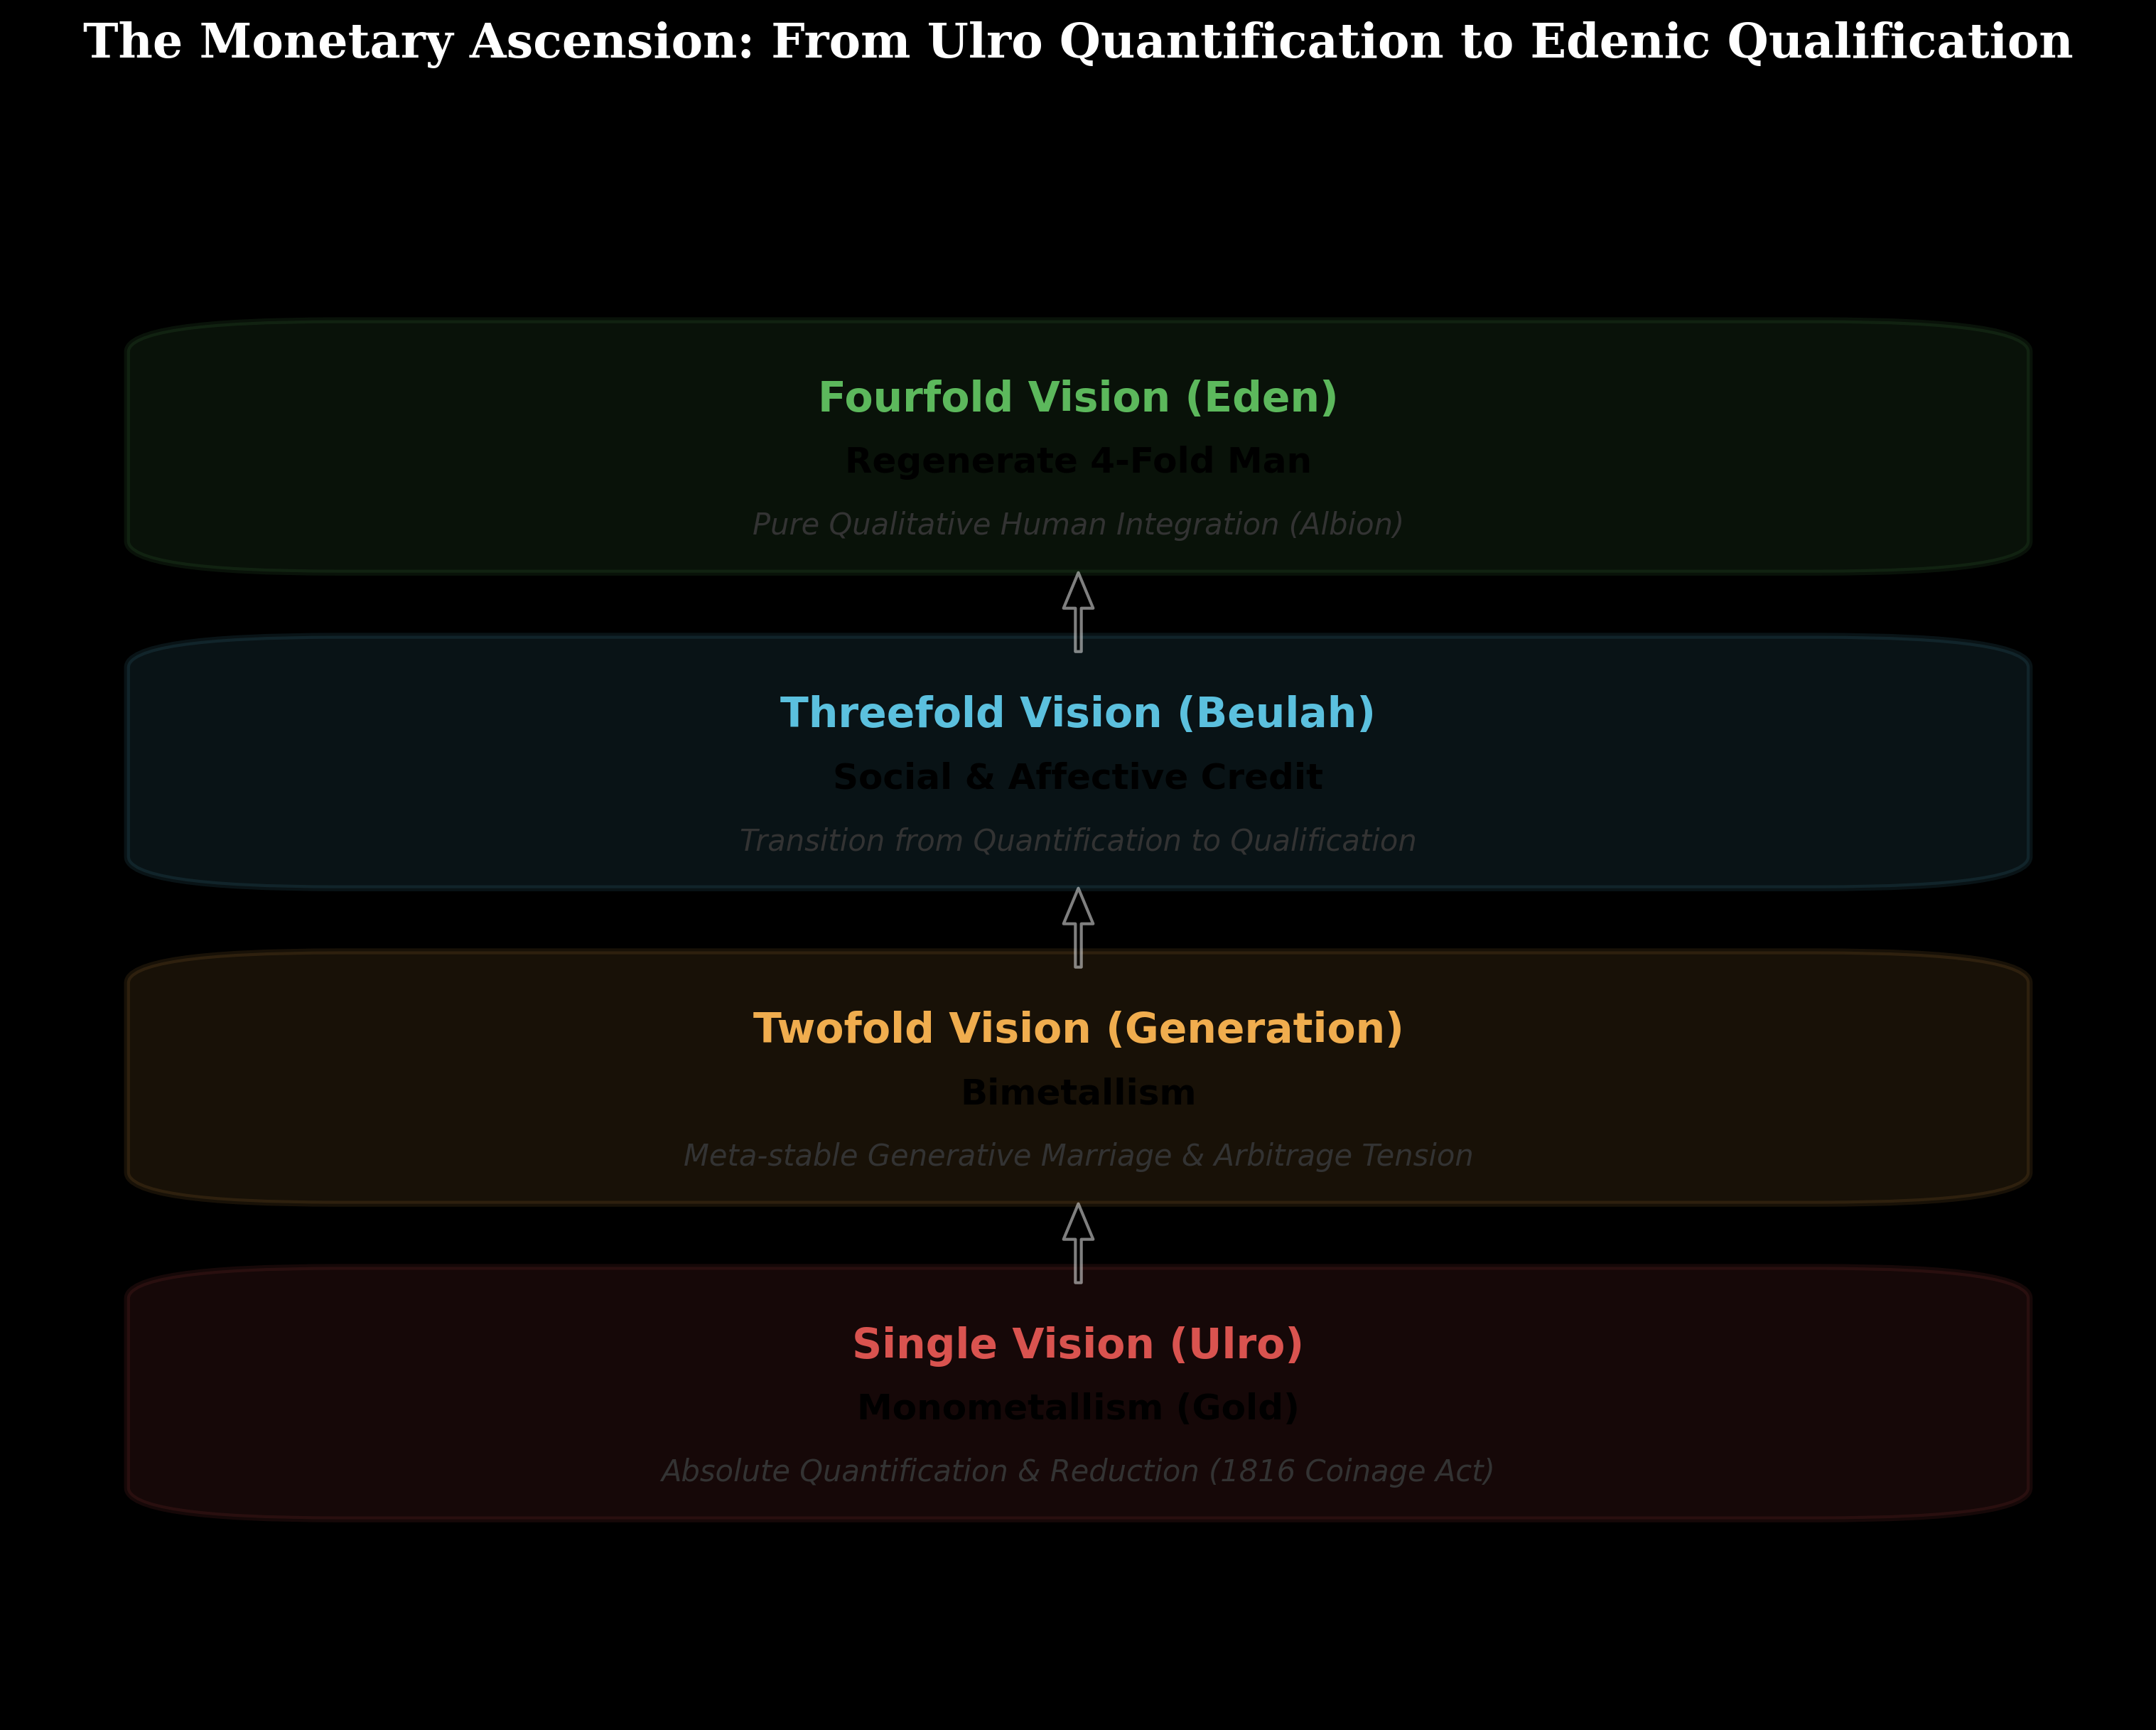
\includegraphics[keepaspectratio,alt={The Monetary Ascension --- From Ulro to Eden. A four-tiered ontological mapping elevating from the reductionist Monometallic standard of Ulro (Single Vision) through the generative bimetallic tension of Generation (Twofold Vision), the affective threshold of Beulah (Threefold Vision), and culminating in the non-dual qualitative integration of the Edenic state (Fourfold Vision). Each tier maps directly onto a specific historical monetary regime, from the sterile finality of the 1816 Gold Standard (Ulro) to the visionary artisanal economics embodied in Los's forge (Eden). This progression provides a critical topological heuristic for reading Blake's late epics: the journey out of the fallen world is not an escape from materiality, but an ascension through increasingly complex architectures of socio-economic relationality.}]{../figures/fourfold_mapping.png}}
\caption{The Monetary Ascension --- From Ulro to Eden. A four-tiered
ontological mapping elevating from the reductionist Monometallic
standard of Ulro (Single Vision) through the generative bimetallic
tension of Generation (Twofold Vision), the affective threshold of
Beulah (Threefold Vision), and culminating in the non-dual qualitative
integration of the Edenic state (Fourfold Vision). Each tier maps
directly onto a specific historical monetary regime, from the sterile
finality of the 1816 Gold Standard (Ulro) to the visionary artisanal
economics embodied in Los's forge (Eden). This progression provides a
critical topological heuristic for reading Blake's late epics: the
journey out of the fallen world is not an escape from materiality, but
an ascension through increasingly complex architectures of
socio-economic relationality.}\label{fig-fourfold}
\end{figure}

\newpage

\section{The Alchemical Forges: Los vs.~The Royal
Mint}\label{the-alchemical-forges-los-vs.-the-royal-mint}

If Urizen is the bureaucratic Master of the Mint---the Newtonian
administrator calculating ratios, imposing geometric limits, and
standardizing the infinite human soul into weighed coins---then Los is
the divine blacksmith, the alchemist of the spirit. The opposition
between these two figures encodes one of the most structurally coherent
economic critiques in the entire Romantic canon.

\subsection{The Mint on Tower Hill: Engines of
Homogenization}\label{the-mint-on-tower-hill-engines-of-homogenization}

In \emph{Jerusalem}, Los is constantly depicted laboring at his roaring
furnaces. Blake utilizes explicitly metallurgical and alchemical imagery
to describe this work. However, whereas the Royal Mint on Tower
Hill---relocated in 1810 to a purpose-built facility on Little Tower
Hill designed by James Johnson and Robert Smirke---was an industrial
fortress of steam-powered homogenization, Los's forges are designed to
produce living, differentiated, irreducibly unique human forms (Eden).
The Mint's industrial transformation was itself a symptom of the
Urizenic revolution: Matthew Boulton's steam-powered coining presses,
installed at the Soho Mint in Birmingham and later adopted at the Royal
Mint, could strike coins with mechanical precision at high speed,
eliminating the human hand from the minting process entirely and
replacing the artisan's judgment with calibrated, replicable force.

The Mint melts down the various, chaotic silver and gold of the world
and stamps it with the sovereign's head---a singular image of authority.
It is a process of extraction and homogenization that parallels exactly
the Urizenic cosmogony described in \emph{The First Book of Urizen}
(1794), where the tyrant ``form'd golden compasses / And began to
explore the Abyss'' \citep{blake1795urizen}. Los's furnaces, conversely,
operate on a principle of spiritual alchemy: taking the fragmented,
degraded, atomic material of the fallen world and fusing it back
together through the heat of prophetic imagination into the ``Human Form
Divine.'' This opposition encodes a fundamental first-principles insight
into the nature of value itself: the Mint's operation is
\emph{subtractive} (reducing diverse human labor to a single metallic
denominator), whereas Los's forge is \emph{additive} (synthesizing
fragmented experience into integrated wholes).

The metallic imagery in \emph{Jerusalem} is pervasive and deliberate. On
Plate 12, Blake describes the spiritual architecture of
Golgonooza---Los's prophetic city, the anti-London---in explicitly
metallurgical terms:

\begin{quote}
``The stones are pity, and the bricks, well wrought affections, Enameld
with love \& kindness, \& the tiles engraven gold, Labour of merciful
hands: the beams \& rafters are forgiveness: The mortar \& cement of the
work, tears of honesty: the nails, And the screws \& iron braces, are
well wrought Blandishments'' (\emph{Jerusalem}, Plate 12, lines 30--34;
Erdman p.~155) \citep{erdman1988complete}
\end{quote}

Here the ``tiles engraven gold'' and ``iron braces'' serve a function
opposed to the Mint's gold: they are construction materials for a city
built from human affect---pity, kindness, forgiveness, honesty---rather
than the weight of bullion. Further, on the same plate, Blake names
``the golden Looms of Cathedron'' and ``the golden mills of Los'' (Plate
12, lines 46--47; Erdman p.~156), establishing that Los possesses his
own golden instruments, but ones devoted to weaving and milling the
fabric of human reality rather than stamping coins of abstract
equivalence. The adjective ``golden'' in Blake is thus bifurcated:
Urizen's gold is dead and hoarded; Los's gold is living, laboring, and
regenerative.

\subsection{The Boulton Press and the Artist's
Body}\label{the-boulton-press-and-the-artists-body}

Blake explicitly contrasts the mechanical, steam-powered presses of
early industrial capitalism---embodied most visibly by the Boulton steam
presses---with the vital, bodily labor of the artist. The production of
true value requires sweat, breath, and the integrated labor of the
entire human body, not the alienated pull of a lever. As Thompson
documents, Blake's hostility to industrial machinery was not Luddite
nostalgia but a precise philosophical objection: the machine severs the
connection between the laborer's creative will and the product of their
hands, reproducing the structure of Urizenic alienation at the level of
daily lived experience \citep{thompson1993witness}.

\begin{quote}
``And Los's Furnaces howl loud; living: self-moving: lamenting With Fury
\& Despair, \& they dictate the relations of States'' (\emph{Jerusalem},
Plate 73) \citep{erdman1988complete}
\end{quote}

The furnaces are not inert mechanisms; they are \emph{living},
\emph{self-moving}, \emph{lamenting}---they participate in the suffering
of the human condition even as they labor to transcend it. This is
Blake's radical proposition: that the sites of genuine
production---artistic, spiritual, political---are necessarily sites of
anguish and fury, not the automated efficiency of the Mint.

\subsection{The Anti-Coin: Blake's Illuminated Printing as Economic
Subversion}\label{the-anti-coin-blakes-illuminated-printing-as-economic-subversion}

For Blake, the true economy is not dictated by the Bank of England or
the bullion brokers of the Royal Exchange, but by the ``Furnaces of
Los.'' The artist's labor---specifically Blake's invention of
illuminated printing via relief-etching (c.~1788)---becomes the only
valid site of socio-metaphysical reproduction. Blake's relief-etching
process is the economic inverse of the Mint's stamping dies: where
Newton's Urizenic 1717 Great Recoinage \emph{stamped} an image of
sovereign authority onto a blank disc to impose fungible value, Blake
\emph{dissolved} the surface of the copper plate with acid to reveal a
unique, irreproducible spiritual topography. The Mint standardizes the
infinite human soul into fixed bimetallic weights; Blake's acid bath
frees the living form from the dead copper. Each illuminated plate is an
anti-coin: singular, non-fungible, resistant to the metric logic of
exchange \citep{poovey2008genres}. Its value does not inhere in the
weight of its copper but in the density of the visionary experience it
encodes.

The choice facing humanity is clear: be minted as a passive coin under
Urizen, or forge one's own infinite value in the roaring fires of Los
\citep{blake1804jerusalem}. As Erdman argues, this is not merely
artistic preference but political economy: Blake's mode of production
constitutes a complete alternative to the industrial system, one in
which the producer retains full sovereignty over the means, process, and
meaning of their labor \citep{erdman1954prophet}.

\newpage

\section{Quantification into
Qualification}\label{quantification-into-qualification}

\subsection{Illuminated Nonduality and the Fourfold
Vision}\label{illuminated-nonduality-and-the-fourfold-vision}

Meta-stability inevitably ruptures, as demonstrated by the arbitrage of
Gresham's Law. But for Blake, rupture is not the end; it is the
threshold marking the transition from the tensions of \textbf{Generation
(Twofold Vision)} and \textbf{Beulah (Threefold Vision)} into the
liberation of \textbf{Eden (Fourfold Vision)}: the realization of the
``regenerate 4-fold man.''

\subsubsection{The Telos of Fourfold
Integration}\label{the-telos-of-fourfold-integration}

This eschatological pivot demands the abandonment of Urizenic
\emph{Quantification} (see the
\href{03b_los_and_fourfold_vision.md\#the-four-levels-of-monetary-vision-and-generation}{overview
of the Four Levels of Vision}) in favor of infinite, boundless
\emph{Qualification}. As Northrop Frye elucidates in his foundational
work \emph{Fearful Symmetry}, Fourfold Vision represents Blake's
ultimate philosophical and spiritual telos: it is imaginative creativity
operating as a living, breathing power, restoring the fractured human
form, Albion \citep{frye1947fearful}. In Blake's mythology, Albion is
simultaneously the primal human, the island of Britain, and the totality
of human civilization---his restoration is therefore at once a personal,
political, and cosmic event. In a truly Fourfold economic system, value
is no longer an intrinsic elemental property mysteriously inhering in
dead base matter (like the weight of gold bullion in a bank vault) or
fictional ledgers of compounding usury. Value becomes exclusively an
emergent property of qualitative, active, synergetic human integration.
It exists strictly within the context of radical human engagement---what
Saree Makdisi characterizes as Blake's ``rewrite'' of the material
capitalist order \citep{makdisi2003william}.

\subsubsection{The Anti-Coin: Relief Etching as Economic
Praxis}\label{the-anti-coin-relief-etching-as-economic-praxis}

This subversion of capitalist order is not merely thematic in Blake's
work; it is structurally embedded in his very mode of production:
illuminated printing. By inventing and operating his hybrid form of
relief etching---biting words and images simultaneously into corrosive
copper baths in a single, nondual matrix---Blake physically achieved a
Fourfold qualitative synthesis in his own life. The copperplate becomes
the anti-coin. Whereas the Royal Mint stamps an image of state authority
onto a blank disc to impose monolithic, fungible value---a process
accelerated to industrial scale by Boulton's steam presses---Blake
dissolved the blank surface of the copper with acid to reveal a unique,
irreproducible spiritual topography. Each illuminated plate cost Blake
not the weight of its metal but the expenditure of his creative
attention: hours of drawing, writing, etching, printing, and
hand-coloring that could never be mechanically replicated.

\subsubsection{The Fusion of Temporal, Spatial, and Sculptural
Labor}\label{the-fusion-of-temporal-spatial-and-sculptural-labor}

The illuminated book seamlessly fuses poetry (temporal), visual art
(spatial), and physical labor (sculptural etching) into a single
artifact that defies the Urizenic division of labor. As Thompson argues,
the division of labor was the central mechanism of industrial
capitalism's alienation of the worker, and Blake's illuminated printing
constitutes a deliberate, material refusal of this division
\citep{thompson1993witness}. Blake took disparate, base elements and
united them in an unstable medium that is sustained entirely by the
human attention and interaction of the reader, demanding active,
Fourfold engagement to decode its sprawling mythological architecture.
The reader of an illuminated book cannot be a passive consumer---the
text demands interpretive labor, visual attention, and imaginative
participation simultaneously. This is the economic logic of Eden applied
to the act of reading itself.

Blake proved, through the very medium of his craft, that true and
lasting value is generated not by the metallic anchor overseen by Sir
Isaac Newton, nor the ``allegoric riches'' of the Bank Restriction, but
by the ``regenerate 4-fold man'' acting in imaginative societal synergy.
Through relief etching, Blake literally minted a new currency of the
spirit, one essentially immune to the entropic arbitrage of the
bimetallic world. As Blake declares in \emph{Milton}: ``Leave counting
Gold \& diamonds, for Gods eye delights in thee'' (Plate 26, line 27;
Erdman p.~121) \citep{erdman1988complete}---the injunction to abandon
the dead metrics of Urizen in favor of the infinite valuations of the
divine imagination.

\newpage

\section{The 1816 Coinage Act as Topological
Regression}\label{the-1816-coinage-act-as-topological-regression}

While Blake proposed a visionary resolution to the meta-stable friction
of Twofold Generation through infinite, Fourfold spiritual expansion,
the British state pursued the exact opposite trajectory. Reacting
against both the swerve of unbacked paper money (see
\href{02c_bank_restriction_1797.md\#the-1797-bank-restriction-and-the-suspension-of-metallic-reality}{the
1797 Bank Restriction}) and the arbitrage of the bullion trade, the
government sought a rigid anchor.

\subsection{Lord Liverpool's Act: The Legislative Architecture of
Monometallism}\label{lord-liverpools-act-the-legislative-architecture-of-monometallism}

Under the guidance of Lord Liverpool, Parliament passed the Coinage Act
of 1816 (56 Geo. III c.68) on \textbf{22 June 1816}, officially known as
``An Act to provide for a New Silver Coinage, and to regulate the
Currency of the Gold and Silver Coin of this Realm.'' This Act legally
demonetized full-bodied silver entirely as a standard of value. It
relegated silver to a mere token coinage---reduced in weight to 66
shillings per troy pound from the prior 62 shillings, and declared legal
tender only for amounts up to \textbf{40 shillings}---effectively ending
the bimetallic alchemical marriage of the previous centuries and
enforcing a strict \emph{de jure} Gold Standard
\citep{redish1990evolution}. The new gold sovereign was defined at
\textbf{123.274 grains} (7.988 grams) of standard \textbf{22-carat gold}
(91.67\% pure), with one troy pound of standard gold equivalent to
\textbf{£46 14s 6d} (44½ guineas). This sovereign coin would become the
foundation of British imperial finance for a century.

\subsection{The Mathematical Necessity of
Collapse}\label{the-mathematical-necessity-of-collapse}

The mathematical necessity of this collapse is formalized by Velde's
border conditions for bimetallism. For both metals to circulate
concurrently, the global commodity price ratio (\(P_G^G / P_G^S\)) must
dynamically satisfy strict world monetary demand shares (\(m_G, m_S\)):

\begin{equation}
\label{eq:velde_demand_shares}
m_G (1 - m_G) < \frac{P_G^G}{P_G^S} < \frac{(1 - m_S)}{m_S}
\end{equation}

By legally tokenizing silver (\(m_S \to 0\) as a standard of sovereign
reserve), the 1816 Coinage Act intentionally violated this inequality,
mathematically engineering a permanent structural singularity
\citep{velde2005bimetallism, quinn1996competing}. Lord Liverpool and the
architects of the Act did not ``resolve'' the crisis of human value;
rather, from a Blakean perspective, they triggered a topological
regression back into the quantification of \textbf{Single Vision
(Ulro)}.

\subsection{The Chimeric Regime and the Amputation of
Silver}\label{the-chimeric-regime-and-the-amputation-of-silver}

As Joseph Albernaz theorizes in his work on common wealth, totalizing
measurement regimes like the Gold Standard operate as deeply
``chimeric'' technologies. They enforce false ontologies to ``ground'' a
community, purposefully obfuscating humanity's shared
``groundlessness''---our fundamental interdependence
\citep{albernaz2024common}. The 1816 Act was the finalized Urizenic
framing of the British economy. The esoteric bimetallic tension (Twofold
Vision) was erased not by synthesizing gold and silver into a higher
qualitative order of human flourishing, but by amputating the lunar
element of silver entirely. By tying the productive capacity of the
British Empire to one isolated, calculable element---the 22-carat
sovereign---the state surrendered to the condition where nothing exists
unless it can be mathematically derived from gold. The social
consequences were severe: as Del Mar documents, the contraction of the
monetary base that followed silver's demonetization enriched the
creditor class while plunging the producing classes into deflationary
poverty---a transfer of wealth from labor to capital that Blake's
\emph{Jerusalem} had prophetically condemned as the ``curb / Of Poverty
on the laborious'' \citep{delmar1895history, erdman1988complete}.

\begin{figure}
\centering
\pandocbounded{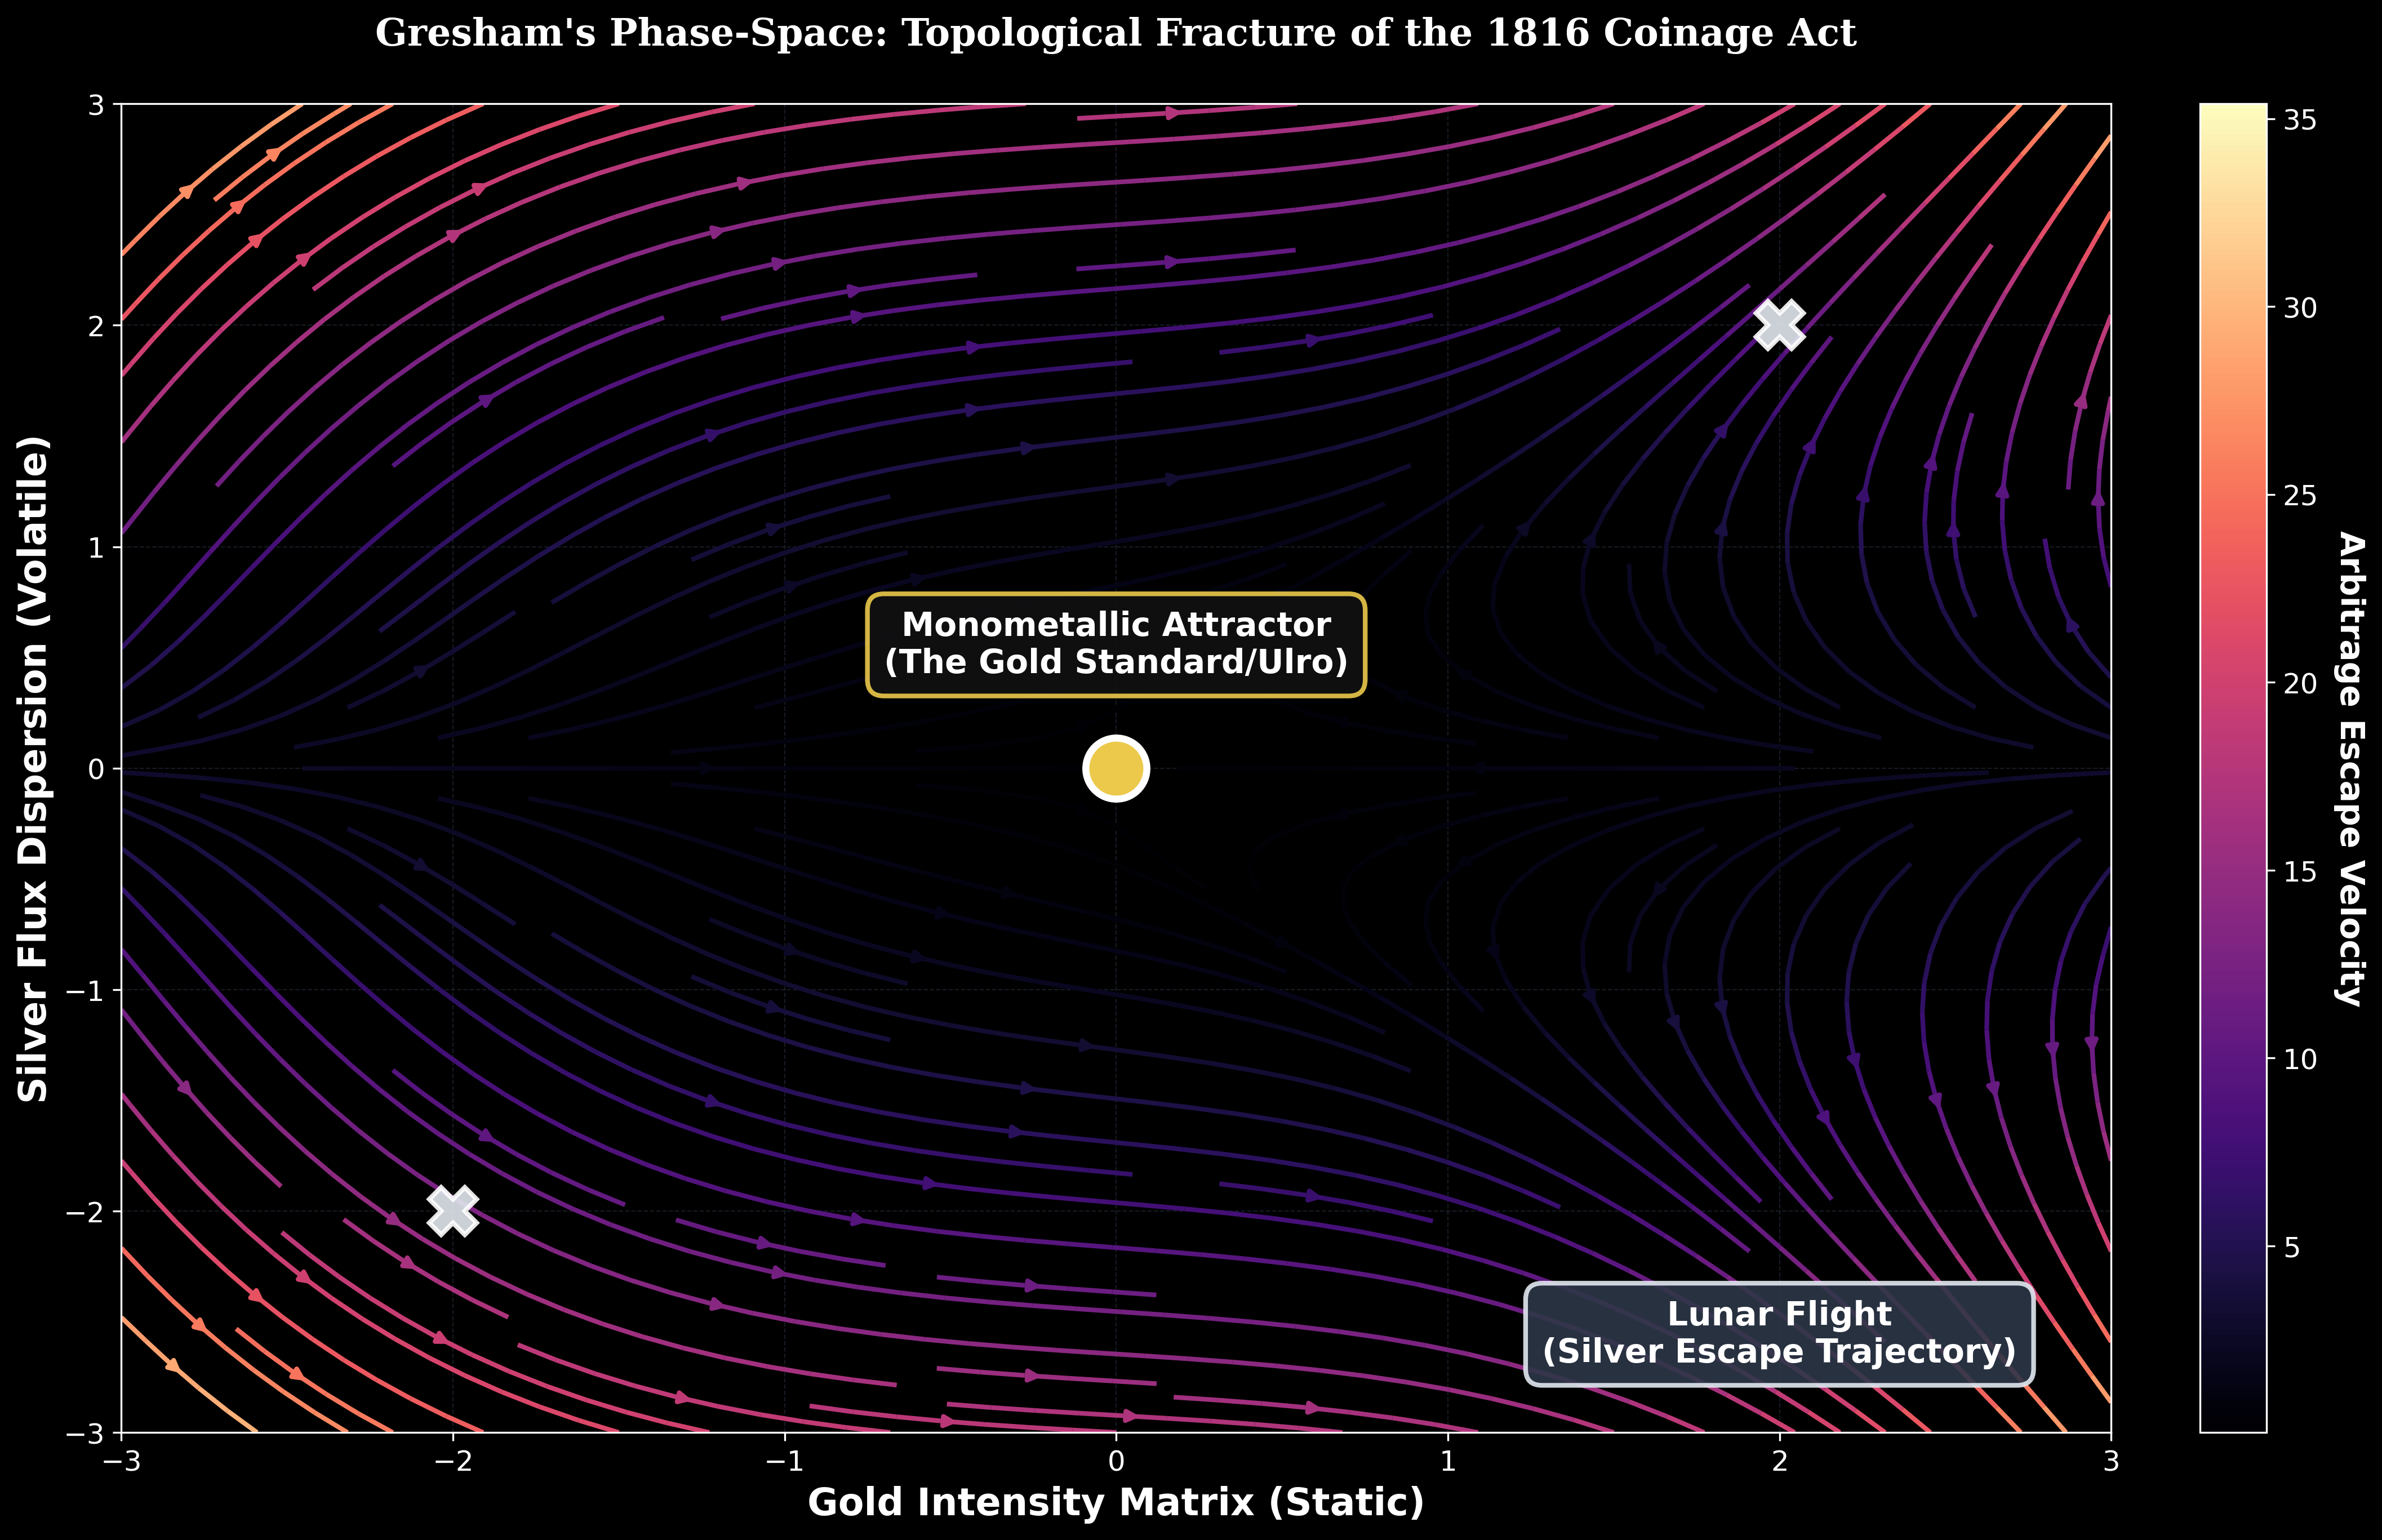
\includegraphics[keepaspectratio,alt={Topological Fracture of Gresham's Law in Phase-Space. This dynamic magma streamplot visualizes the macroeconomic collapse of bimetallic metastability, driven by the bounding inequality m\_G(1 - m\_G) \textless{} \textbackslash frac\{P\_G\^{}G\}\{P\_G\^{}S\} \textless{} \textbackslash frac\{(1 - m\_S)\}\{m\_S\}. The geometric center (Gold Attractor, m\_S \textbackslash to 0 / Ulro / 1816 Singularity) exerts an inflexible inward-pulling vector field (U = -X + 2Y\^{}2)---the gravitational well of the monometallic standard: the 22-carat sovereign at 123.274 grains freezing human exchange into static atoms of sovereign credit. The outward thermal-gradient vectors represent the Lunar Flight (V = 0.5Y + YX\^{}2): silver arbitrage shattering its state-mandated bond. As the Mint Ratio (M) diverges structurally from the international Market Ratio (R)---Newton's 1:15.21 against the European market's 1:14.5---the currency system undergoes topological clinamen. The 1816 Coinage Act enforced the terminal Urizenic amputation of silver, restricting token coinage to 40 shillings.}]{../figures/topological_fracture.png}}
\caption{Topological Fracture of Gresham's Law in Phase-Space. This
dynamic magma streamplot visualizes the macroeconomic collapse of
bimetallic metastability, driven by the bounding inequality
\(m_G(1 - m_G) < \frac{P_G^G}{P_G^S} < \frac{(1 - m_S)}{m_S}\). The
geometric center (Gold Attractor, \(m_S \to 0\) / Ulro / 1816
Singularity) exerts an inflexible inward-pulling vector field
(\(U = -X + 2Y^2\))---the gravitational well of the monometallic
standard: the 22-carat sovereign at 123.274 grains freezing human
exchange into static atoms of sovereign credit. The outward
thermal-gradient vectors represent the Lunar Flight
(\(V = 0.5Y + YX^2\)): silver arbitrage shattering its state-mandated
bond. As the Mint Ratio (\(M\)) diverges structurally from the
international Market Ratio (\(R\))---Newton's 1:15.21 against the
European market's 1:14.5---the currency system undergoes topological
clinamen. The 1816 Coinage Act enforced the terminal Urizenic amputation
of silver, restricting token coinage to 40
shillings.}\label{fig-topology}
\end{figure}

\subsection{The Victory of ``Single Vision \& Newton's
Sleep''}\label{the-victory-of-single-vision-newtons-sleep}

This systemic reduction was the ultimate victory of ``Single vision \&
Newtons sleep'' (as Blake declared in his 1802 letter to Butts; Erdman
p.~722) \citep{erdman1988complete}. It represented a reduction of the
regenerate 4-fold man back into an isolated, atomized economic cog,
evaluated solely against the geometric weight of the new golden
sovereign coin. It was a regression into intellectual and spiritual
infancy under the guise of scientific finance, establishing a paradigm
of scarcity that Blake would fight until his last breath. The arc from
Newton's 1717 ratio through the 1797 Restriction to the 1816 Act traces
a complete Blakean narrative: from the imposition of Urizenic geometry
upon the living economy, through the chaotic void of paper abstraction,
to the final re-assertion of monometallic control. Blake's prophetic
response---the immense, unfinished architecture of \emph{Jerusalem},
composed across exactly these years---constitutes the most sustained
imaginative resistance to this economic ontology in the entire literary
canon.

\newpage

\section{Esoteric Finance: Blake and Alexander Del
Mar}\label{esoteric-finance-blake-and-alexander-del-mar}

If William Blake provided the visionary, mythopoetic critique of
18th-century monetary metaphysics, the late 19th-century historian
Alexander Del Mar provided its rigorous historiographical counterpart.
Del Mar's \emph{History of Monetary Systems} (1895) operates on a
fundamental thesis that maps onto Blakean cosmology: that the right to
coin money is a sovereign, communal prerogative (a state of Edenic or at
least Beulah-like integration) that has been recurrently hijacked
throughout history by private, atomizing mercantile interests (Urizen)
\citep{delmar1895history}.

\subsection{The Sacred Prerogative of
Issuance}\label{the-sacred-prerogative-of-issuance}

For Del Mar, the ``esoteric'' aspect of finance is precisely this hidden
historical struggle over the prerogative of issuance. When the state
controls the money supply, value is derived from the \emph{societal
totality} (the Human Form Divine) and the collective needs of the
people. When private banks (such as the Bank of England in 1797) or
rigid metallic ratios (Newton in 1717, Liverpool in 1816) assume
control, value is transferred to the dead material of the coin itself or
the fictional ledger of the private creditor \citep{clapham1944bank}.
Del Mar writes extensively on the sacred, often solar and lunar origins
of coinage in antiquity, viewing the bimetallic system not as an
economic expedience, but as a degraded remnant of a dualistic religious
system representing divine authority. The golden disc and the silver
crescent encoded, in the earliest Mesopotamian and Egyptian monetary
systems, the solar and lunar principles that governed all legitimate
sovereignty---a thesis that reveals the transition from bimetallism to
the gold standard not merely as a policy adjustment but as a
metaphysical revolution: the displacement of a dualistic, syncretic
cosmology by a monistic, reductionist one. This perspective illuminates
a \emph{generic} economic principle: every monetary regime encodes a
specific theology of value.

\subsection{Blake's Jerusalem Plate 10 and the Architecture of
Enslavement}\label{blakes-jerusalem-plate-10-and-the-architecture-of-enslavement}

Blake recognized this identical usurpation with prophetic clarity. His
condemnation of the Bank of England, the Mint, and the gold standard was
rooted in his understanding that whoever controls the semiotics of value
controls the human soul. Blake's famous declaration:

\begin{quote}
``I must Create a System, or be enslav'd by another Mans I will not
Reason \& Compare: my business is to Create'' (\emph{Jerusalem}, Plate
10, lines 20--21; Erdman p.~153) \citep{erdman1988complete}
\end{quote}

is precisely this recognition that the \emph{architecture} of
representation determines the freedom or subjugation of human life. The
``System'' Blake must create is not merely a mythological schema but an
entire alternative regime of valuation---one grounded in the irreducible
particularity of creative labor rather than the abstract universality of
the gold sovereign. When Del Mar catalogs the social consequences of the
demonetization of silver---how the contraction of the monetary base
enriched the creditor class while plunging the producing classes into
deflationary poverty---he is documenting the literal effects of Urizen's
``brazen quadrant'' upon the British and global economy
\citep{delmar1885history}.

\subsection{The 1844 Bank Charter Act and the Ledger Migration of
Spectral
Value}\label{the-1844-bank-charter-act-and-the-ledger-migration-of-spectral-value}

The culmination of this architectural subjugation occurred with the 1844
Bank Charter Act (Peel's Act). The fiercely contested debate between the
Banking School and the Currency School was ultimately resolved when
Parliament centralized all note issuance under the Bank of England's
strict monopoly, tying paper currency to a 100\% gold reserve above a
fixed fiduciary minimum. The Currency School theorists, acting as the
ultimate architects of Urizenic geometry, believed they had finally
imprisoned the chaos of economic swerve within the immutable
predictability of the gold standard.

However, by focusing on paper notes, Peel's Act paradoxically ignored
the explosive growth of bank deposits and ledger credit, which rapidly
emerged to comprise 90\% of the money supply in late 19th-century
Britain. The ``fictive'' or ``spectral value'' against which Blake raged
did not vanish; rather, the ``ghosts'' completely migrated out of the
physical paper artifact and into the invisible, unregulated abstraction
of the bank ledger. This endogenous expansion of invisible credit
represents a profound esoteric mutation of the capitalist economy---a
system sustained entirely by mathematical promises that periodically
collapsed in late-century panics.

\subsection{The Convergence of Prophetic and Historiographic
Critique}\label{the-convergence-of-prophetic-and-historiographic-critique}

Both Blake and Del Mar understood that the true ``alchemy'' of money had
been stolen from the domain of human creativity. The living, breathing
economy of human interaction had been replaced by a spectral, numerical
simulation engineered to perpetually enrich the creditor class at the
direct expense of the producing masses. Reading Blake through the lens
of esoteric finance elevates his poetic epics from obscure mystical
allegories into profound critiques of modern central banking and
financialized alienation \citep{poovey2008genres, baucom2005specters}.
Del Mar's key historiographic insight---that the demonetization of
silver was a deliberate political act designed to redistribute wealth
upward---finds its mythopoetic expression in Blake's \emph{Jerusalem},
where the architects of financial enclosure are exposed as agents of
Urizenic tyranny.

By demanding in \emph{Milton} that humanity ``Leave counting Gold \&
diamonds, for Gods eye delights in thee'' (Plate 26, line 27; Erdman
p.~121) \citep{erdman1988complete}, Blake stands alongside Del Mar as a
prophet declaring that the highest sovereign act is not the balancing of
a metallic ratio, but the liberation of the human imagination from the
ledger. Where Del Mar provides the forensic historiography, Blake
provides the visionary horizon: together, they articulate a complete
esoteric economics of human liberation.

\newpage

\section{The Atlantic Crucible: American Bimetallism and the
Architecture of Republican
Money}\label{the-atlantic-crucible-american-bimetallism-and-the-architecture-of-republican-money}

In 1793---the same year the British state declared war on revolutionary
France, the same year radical publishers were arrested under Pitt's
sedition laws---William Blake etched \emph{America A Prophecy} on
eighteen copper plates in his Lambeth workshop. Blake was no isolated
mystic: David Erdman documents that he moved through the radical circles
of 1790s London, frequenting the weekly dinners at Joseph Johnson's
bookshop in St Paul's Churchyard alongside Mary Wollstonecraft, William
Godwin, and Thomas Paine \citep{erdman1954prophet}. When the Pitt
government issued a warrant for Paine's arrest for seditious libel after
\emph{Rights of Man} (1791--92), Blake personally warned Paine, enabling
his escape to France (Erdman p.~200). The poem that emerged from this
milieu presents the American Revolution not as a political event but as
a cosmic conflagration: the unchaining of Orc, the spirit of
revolutionary energy, against the tyranny of Urizen's law. But
\emph{America A Prophecy} is not merely a poem about political
revolution; it is, when read alongside the concurrent monetary crises of
both Britain and the newly constituted United States, a prophetic
meditation on the fundamental relationship between monetary sovereignty,
human freedom, and the architecture of value itself.

\subsection{The Coinage Act of 1792: Hamilton's Republican
Experiment}\label{the-coinage-act-of-1792-hamiltons-republican-experiment}

On 2 April 1792---one year before Blake etched
\emph{America}---President George Washington signed the Coinage Act of
1792, establishing the United States Mint in Philadelphia and codifying
a bimetallic standard with a gold-to-silver ratio of \textbf{15:1}
\citep{laughlin1898bimetallism}. This ratio, proposed by Treasury
Secretary Alexander Hamilton in his \emph{Report on the Establishment of
a Mint} (1791), was itself an act of deliberate divergence from Newton's
British ratio of 1:15.21 \citep{hamilton1791report}. Hamilton explicitly
calculated his ratio by surveying average European market conditions,
aiming for a standard that would attract both metals into domestic
circulation rather than suffer the asymmetric drainage that plagued
Britain \citep{sylla2011hamiltons}. The silver dollar was defined at
\textbf{371.25 grains of pure silver}; the gold eagle at \textbf{247.5
grains of pure gold}. As Richard Sylla and David Cowen demonstrate,
Hamilton's financial architecture---encompassing the Mint, the First
Bank, and the systematic funding of revolutionary war debt---was the
most ambitious experiment in republican finance the modern world had yet
attempted \citep{sylla2011hamiltons}.

This legislative act was revolutionary in its monetary implications, yet
it carried a structural flaw that would destabilize the American economy
for a century. Where Newton's Mint had served the Crown's imperial
prerogative---calibrating a 15.21:1 ratio that systemically overvalued
gold and drained England of silver---Hamilton designed his 15:1 ratio
for a republican experiment in dual-metal equilibrium. However, as
Angela Redish demonstrates in \emph{Bimetallism: An Economic and
Historical Analysis}, Hamilton's flatter ratio sat blindly ``on the
slope of a declining value of silver relative to gold,'' driven by an
oversupply from Latin American mines \citep{redish2000bimetallism}.
Consequently, Hamilton inadvertently overvalued silver. This triggered
Gresham's Law in reverse: gold coins were melted and exported to Europe
where they commanded a higher premium, leaving the United States on a
\emph{de facto} silver standard by 1834. As Lawrence Officer calculates,
the U.S. Mint earned substantial seigniorage profit from the operation
of the bimetallic system despite its structural instability, suggesting
the arrangement served fiscal as well as monetary purposes
\citep{officer2001bimetallism}. Milton Friedman and Anna Schwartz later
analyzed this initial miscalibration as guaranteeing the monetary
volatility that would define 19th-century America
\citep{friedman1963monetary}. Curtis Nettels' study of the early
national economy confirms that Hamilton's system, however flawed in its
ratio, succeeded in establishing the institutional architecture---Mint,
Treasury, funded debt---upon which American monetary sovereignty would
depend \citep{nettels1962emergence}.

Blake's Orc, breaking free from his chains on the Atlantean mountains,
embodies precisely this revolutionary energy. The Preludium to
\emph{America} (Plates 1--4) depicts Orc's liberation as an elemental
eruption: the ``hairy youth'' bursts his chains in a subterranean
cavern, his body burning with the fire of revolutionary desire (Erdman
pp.~51--52) \citep{erdman1988complete}. When we read this mythological
unchaining alongside the simultaneous establishment of a new monetary
sovereign---a nation explicitly rejecting the Bank of England's
monopoly, the Crown's prerogative of issuance, and the Newtonian
metrological regime---Orc's fire becomes legible as the liberation of
value itself from the calculus of empire.

\subsection{Hamilton vs.~Jefferson: The Structural Antinomy of
Republican
Finance}\label{hamilton-vs.-jefferson-the-structural-antinomy-of-republican-finance}

The American experiment in bimetallism was, from its inception, riven by
an internal antinomy that maps with remarkable precision onto Blake's
mythological framework. Alexander Hamilton---the architect of the First
Bank of the United States (chartered 1791)---envisioned a centralized
financial architecture modeled on, though deliberately constrained
relative to, the Bank of England. Hamilton's bank, capitalized at \$10
million, was authorized to issue banknotes, manage federal debt, and
coordinate fiscal policy---functions that Thomas Jefferson viewed as a
direct assault on republican agrarian virtue
\citep{laughlin1898bimetallism, wilentz2005rise}.

Jefferson's opposition to the Bank was not merely constitutional (though
he argued strenuously that the Constitution granted no power to charter
a federal bank); it was ontological. Jefferson insisted that the
productive labor of the farmer---the physical working of the
earth---constituted the only legitimate foundation of national wealth.
Paper credit, fractional reserve banking, and the abstractions of urban
finance were, in Jefferson's view, parasitical fictions that enriched
speculators at the expense of the producing classes. As Sean Wilentz
documents in \emph{The Rise of American Democracy}, this
Hamilton-Jefferson divide defined the fundamental fault line of American
political economy for the next century, structuring every subsequent
conflict over banking, tariffs, and monetary standards
\citep{wilentz2005rise}. This position resonates with Blake's
condemnation of ``allegoric riches'' (\emph{Jerusalem}, Plate 27; Erdman
p.~170) \citep{erdman1988complete, sklar2011blake}: both Blake and
Jefferson recognized that the architecture of money creation determined
the distribution of real power and real suffering.

Yet Jefferson's agrarian alternative was itself caught in the
contradictions of commodity production. The Jeffersonian farmer remained
dependent on metallic currency---on the very gold and silver whose
statutory ratios, as Gresham's Law demonstrated, were subject to
international arbitrage beyond any single nation's control. Blake's
prophetic critique extends further than either Hamilton's centralized
finance or Jefferson's agrarian metallist position: for Blake, the
fundamental error is the reduction of value to \emph{any} quantitative
metric, whether gold, silver, or paper. ``Can Wisdom be put in a silver
rod? / Or Love in a golden bowl?'' (\emph{The Book of Thel}, 1789)
\citep{blake1789thel}---this question applies with equal force to
Hamilton's Treasury notes and Jefferson's silver dollars.

\newpage

\section{\texorpdfstring{\emph{America A Prophecy} and the Political
Economy of Revolutionary
Perception}{America A Prophecy and the Political Economy of Revolutionary Perception}}\label{america-a-prophecy-and-the-political-economy-of-revolutionary-perception}

\subsection{``Shaking their mental chains'': Blake's Prophecy at the
Monetary
Threshold}\label{shaking-their-mental-chains-blakes-prophecy-at-the-monetary-threshold}

\emph{America A Prophecy} (1793) is structured in two movements: a
Preludium of mythological unchaining and a Prophecy of revolutionary
confrontation. At its center lies a passage of economic and
epistemological resonance. When the Thirteen Governors convene in
Bernard's house and the flames of Orc engulf the land, the colonial
administrators react with terror:

\begin{quote}
``Shaking their mental chains, they rush in fury to the sea To quench
their anguish; at the feet of Washington down fall'n They grovel on the
sand and writhing lie'' (\emph{America A Prophecy}, Plates 13--14;
Erdman p.~55) \citep{erdman1988complete, blake1793america}
\end{quote}

The phrase ``mental chains'' is Blake's articulation of the relationship
between political subjugation and epistemic imprisonment. These are not
physical manacles but conceptual constraints---the same ``mind-forg'd
manacles'' that Blake would later identify in \emph{London} (Songs of
Experience, 1794; Erdman p.~70) \citep{erdman1988complete}. In the
context of the bimetallic monetary crisis, the ``mental chains'' are the
very statutory ratios, fixed prices, and abstract ledgers that bind
human labor to metallic equivalences. The governors do not merely lose
political authority; they lose the entire conceptual apparatus through
which they have administered value.

\subsection{Boston's Angel and the Commodification of Human
Virtue}\label{bostons-angel-and-the-commodification-of-human-virtue}

The most economically resonant passage in \emph{America} is Boston's
Angel's speech, which Blake positions as the poem's intellectual climax:

\begin{quote}
``Who commanded this? What God? What Angel? To keep the gen'rous from
experience till the ungenerous Are unrestrain'd performers of the
energies of nature; Till pity is become a trade, and generosity a
science That men get rich by; and the sandy desert is giv'n to the
strong?'' (\emph{America A Prophecy}, Plate 9; Erdman p.~53)
\citep{erdman1988complete, blake1793america}
\end{quote}

This passage demands economic exegesis. ``Pity is become a trade''
anticipates by eighty years Karl Marx's analysis of how capitalism
transforms all human relations into commodity relations: even compassion
itself becomes a tradeable asset, a resource to be deployed for profit.
``Generosity a science / That men get rich by'' describes with precision
the logic of speculative philanthropy, charitable endowments, and the
broader financialization of human virtue that was already visible in the
operations of the Bank of England's credit system
\citep{poovey2008genres}. Patrick Brantlinger's \emph{Fictions of State}
traces how this transformation of moral sentiment into financial
infrastructure extended through the entire edifice of 18th-century
credit culture, creating what he terms a ``culture of speculation'' in
which even patriotism and public spirit were securitized
\citep{brantlinger1996fictions}.

As Saree Makdisi argues, Blake's \emph{America} challenges the emerging
commodity-form of perception itself: the idea that knowledge, like
goods, is something passively received from external authority rather
than actively produced through imaginative engagement
\citep{makdisi2003william}. Boston's Angel demands to know \emph{who has
the right to restrict experience}---a question that applies with equal
force to the sovereign's right to fix the price of metal and the Bank's
right to restrict the conversion of paper into gold. Jon Mee's
\emph{Dangerous Enthusiasm} contextualizes Blake within the broader
culture of 1790s radical dissent, demonstrating that Blake's critique of
commodified experience drew directly on the millenarian and antinomian
traditions that informed popular resistance to enclosure, taxation, and
the disciplinary apparatus of Pitt's wartime state
\citep{mee1992dangerous}.

\subsection{The ``Crime'' of 1873 and the Demonetization of
Silver}\label{the-crime-of-1873-and-the-demonetization-of-silver}

Blake's prophetic framework proves its relevance when extended beyond
its immediate historical context to encompass the full arc of American
bimetallic politics. The Fourth Coinage Act of \textbf{12 February
1873}---known to its critics as ``The Crime of 1873''---demonetized the
silver dollar by omitting it from the list of authorized coins,
effectively placing the United States on a gold monometallic standard
\citep{laughlin1898bimetallism}. This legislative act, passed with
little public debate while the nation was still recovering from Civil
War and the Reconstruction crisis, enacted on American soil the same
regression that Blake had diagnosed in Britain's 1816 Coinage Act. As
Richard White documents in \emph{The Republic for Which It Stands}, the
1873 Act was not a sudden conspiracy but the culmination of a
decade-long lobbying campaign by Eastern financial interests who sought
to align American monetary policy with the emerging international gold
consensus centered on London and Berlin \citep{white2017republic}.

The parallels with the British experience are structurally exact. Where
Lord Liverpool's 1816 Act (56 Geo. III c.68) demonetized full-bodied
silver by reducing it to token coinage with a 40-shilling legal tender
limit, the 1873 Act accomplished the same amputation by erasing the
silver dollar from the statute book. As Marc Flandreau argues in
\emph{The Glitter of Gold}, this global shift from bimetallism to gold
was fundamentally a struggle over \emph{political theology}---a contest
between competing visions of what money \emph{is} and whom it should
serve \citep{flandreau2004glitter}. Agrarian producers and Western
miners defended silver as a tangible sacrament of their labor, while
Eastern financial elites demanded the hierarchical, centralized
abstraction of the gold standard. Richard Franklin Bensel's
\emph{Political Economy of American Industrialization} demonstrates that
the deflation following 1873 was not an incidental consequence but a
structural requirement of the gold standard regime, which transferred
wealth systematically from debtor agrarians to creditor financiers
\citep{bensel2000political}.

Where Newton's Mint ratio had overvalued gold to drain England of
silver, the post-1873 deflation---in which Milton Friedman notes
American price levels collapsed by roughly 50\% between 1865 and
1896---crushed American farmers under a contracting gold supply
\citep{friedman1963monetary}. The producing classes of both
nations---the ``laborious'' upon whom Blake's ``Councellor'' throws the
``curb / Of Poverty'' (\emph{Jerusalem}, Plate 27; Erdman p.~170)---bore
the consequences of this monetary contraction, while the urban creditor
class reaped profits from the rising value of their gold-denominated
claims \citep{delmar1895history, erdman1988complete}.

\subsection{The Free Silver Movement and the Populist
Insurgency}\label{the-free-silver-movement-and-the-populist-insurgency}

The political response to the Crime of 1873 constituted nothing less
than the most significant challenge to financial orthodoxy in American
history. The Free Silver movement (1873--1900) demanded the restoration
of free coinage of silver at a ratio of \textbf{16:1}---a deliberate
rejection of the monometallic stranglehold that had impoverished the
agrarian West and South \citep{laughlin1898bimetallism}. Charles
Postel's \emph{The Populist Vision} demonstrates that the Populists were
not, as Richard Hofstadter once dismissively characterized them,
backward-looking agrarian romantics, but sophisticated political actors
who understood the monetary system's structural biases with considerable
analytical precision \citep{postel2007populist, hofstadter1955age}.
Congress responded with the \textbf{Bland-Allison Act of 1878},
requiring the Treasury to purchase \$2--4 million of silver bullion
monthly for coinage, and the \textbf{Sherman Silver Purchase Act of
1890}, mandating the purchase of 4.5 million ounces of silver per
month---legislative interventions that represented partial attempts to
restore the bimetallic synthesis against the crushing monometallism
imposed by Eastern financial interests.

The movement reached its crescendo in William Jennings Bryan's
\textbf{``Cross of Gold'' speech} at the 1896 Democratic National
Convention in Chicago (9 July 1896). As Michael Kazin documents in
\emph{A Godly Hero}, Bryan's address was not merely a political
performance but a distillation of two decades of agrarian rage against
the deflationary regime imposed by the gold standard
\citep{kazin2006godly}. His defense of the agrarian producing classes
against urban financial elites---``You come to us and tell us that the
great cities are in favor of the gold standard; we reply that the great
cities rest upon our broad and fertile prairies. Burn down your cities
and leave our farms, and your cities will spring up again as if by
magic; but destroy our farms and the grass will grow in the streets of
every city in the country''---recapitulates with precision Blake's
insistence that productive, embodied labor constitutes the only true
source of value \citep{laughlin1898bimetallism}. Bryan even invoked the
American Revolution explicitly: ``instead of having a gold standard
because England has, we shall restore bimetallism, and then let England
have bimetallism because the United States have''---a deliberate
re-enactment of 1776's monetary independence.

Bryan's peroration constitutes one of the most powerful expressions of
the critique of monometallism ever uttered in the American political
tradition:

\begin{quote}
``Having behind us the producing masses of this nation and the world,
supported by the commercial interests, the laboring interests, and the
toilers everywhere, we will answer their demand for a gold standard by
saying to them: `You shall not press down upon the brow of labor this
crown of thorns; you shall not crucify mankind upon a cross of
gold.'\,''
\end{quote}

The image of crucifixion upon gold directly inverts the Christian
symbolism that Blake deployed throughout his prophetic works: gold,
which should represent the solar principle of divine love, has been
weaponized into an instrument of torture---the miser's guinea elevated
above the sun until it becomes the cross upon which human labor is
sacrificed. Bryan's speech echoes Blake's demand in \emph{Milton}:
``Leave counting Gold \& diamonds, for Gods eye delights in thee''
(Plate 26, line 27; Erdman p.~121) \citep{erdman1988complete}. Yet Bryan
lost the 1896 election to William McKinley---the candidate of gold and
industrial capital---and the Gold Standard Act of 1900 formally
enthroned the monometallic regime, ending the American bimetallic
experiment that Hamilton had initiated 108 years earlier.

\newpage

\section{Transatlantic Architectures of Monetary Collapse: Britain and
America
Compared}\label{transatlantic-architectures-of-monetary-collapse-britain-and-america-compared}

\subsection{The Divergent Ratios and Their Structural
Consequences}\label{the-divergent-ratios-and-their-structural-consequences}

The British and American bimetallic experiments, though sharing the same
architecture---two metals bound by statutory fiat---diverged in ways
that illuminate both the generic logic of bimetallic instability and the
specific political economies encoded in each nation's monetary regime. A
systematic comparison reveals how Gresham's Law operated with identical
structural logic but divergent political consequences across the
Atlantic.

{\def\LTcaptype{none} % do not increment counter
\begin{longtable}[]{@{}
  >{\raggedright\arraybackslash}p{(\linewidth - 4\tabcolsep) * \real{0.2037}}
  >{\raggedright\arraybackslash}p{(\linewidth - 4\tabcolsep) * \real{0.3704}}
  >{\raggedright\arraybackslash}p{(\linewidth - 4\tabcolsep) * \real{0.4259}}@{}}
\toprule\noalign{}
\begin{minipage}[b]{\linewidth}\raggedright
Parameter
\end{minipage} & \begin{minipage}[b]{\linewidth}\raggedright
Britain (1717--1816)
\end{minipage} & \begin{minipage}[b]{\linewidth}\raggedright
United States (1792--1873)
\end{minipage} \\
\midrule\noalign{}
\endhead
\bottomrule\noalign{}
\endlastfoot
\textbf{Statutory Ratio} & 1:15.21 (Newton, 1717) & 1:15 (Hamilton,
1792); revised to 1:16 (1834) \\
\textbf{Market Reality} & \textasciitilde1:14.5 (European) &
\textasciitilde1:15.5 (European, post-1792) \\
\textbf{Direction of Drainage} & Silver exported to France/India & Gold
exported to Europe (pre-1834); Silver exported (post-1834) \\
\textbf{Central Bank} & Bank of England (1694) & First Bank of US
(1791--1811); Second Bank (1816--1836) \\
\textbf{Suspension Event} & Bank Restriction Act, 27 Feb 1797 &
Greenback suspension, 1862--1879 \\
\textbf{Demonetization} & Coinage Act 1816 (56 Geo. III c.68) & Fourth
Coinage Act, 12 Feb 1873 \\
\textbf{Popular Resistance} & Minimal (no Free Silver equivalent) & Free
Silver movement (1873--1900) \\
\textbf{Prophetic Critique} & Blake's \emph{Jerusalem}, \emph{Milton} &
Bryan's ``Cross of Gold'' (1896) \\
\end{longtable}
}

The table reveals a structural insight: under Hamilton's 15:1 ratio,
which \emph{undervalued} gold relative to the European market of
approximately 15.5:1, the United States initially experienced the mirror
image of Britain's drainage. American gold was exported to Europe where
it commanded higher value, while silver accumulated
domestically---making silver, paradoxically, the \emph{de facto}
American standard through the 1820s
\citep{laughlin1898bimetallism, officer2001bimetallism}. This is
precisely the inverse of Britain's experience under Newton's 15.21:1
ratio, which overvalued gold and drained silver. The 1834 revision to
approximately 16:1 reversed this dynamic, deliberately overvaluing gold
to attract it into domestic circulation---but at the cost of triggering
the same outward silver flight that had devastated British coinage a
century earlier \citep{redish1990evolution}.

\subsection{Jackson's War on the Bank: The Limits of Institutional
Destruction}\label{jacksons-war-on-the-bank-the-limits-of-institutional-destruction}

Andrew Jackson's veto of the Second Bank of the United States in 1832,
followed by his executive removal of federal deposits in 1833 and the
Bank's ultimate demise in 1836, constitute an episode of resonance for
understanding the structural limits of monetary reform. Jackson, the
agrarian populist from the frontier, declared the Bank a ``monopoly''
and a ``hydra of corruption'' that enriched Eastern financial elites at
the expense of the producing classes
\citep{howe2007what, wilentz2005rise}. Daniel Walker Howe's \emph{What
Hath God Wrought} demonstrates that Jackson's Bank War was not merely an
economic dispute but a fundamental contest over the meaning of
democratic sovereignty in the new republic: who should control the
creation of money, and to whose benefit \citep{howe2007what}?

In Blake's mythological terms, this is Orc's revolutionary assault on
the Urizenic institution---the fiery destruction of the centralized
architecture of credit. Yet Jackson's destruction of the Bank unleashed
a ``Free Banking'' era of wildcat state-chartered institutions that
issued unregulated paper currency---precisely the spectral void of
``allegoric riches'' that Blake identified as equally catastrophic. Sean
Wilentz documents how the period between the Bank's destruction (1836)
and the Civil War saw over 1,600 state-chartered banks issuing their own
notes, producing a fragmented, unreliable, and frequently fraudulent
currency system \citep{wilentz2005rise}.

The Jacksonian paradox recapitulates the Blakean diagnosis with
fidelity: destroying the centralized institution does not automatically
produce liberation. In classical political economy terms, Jackson
dismantled the \emph{federal} monopoly on credit only to democratize the
issuance of unbacked paper through state banks---a horizontal
proliferation of the same abstracting technology. Without the
qualitative vision that transcends both metallic fetishism and paper
abstraction, the destruction of one tyranny merely clears the ground for
another. Blake understood this with clarity. As he writes in
\emph{America A Prophecy}, even after Orc's revolutionary fire has
consumed the old order, Urizen descends again:

\begin{quote}
``Urizen, who sat / Above all heavens, in thunders wrapp'd, emerg'd his
leprous head From out his holy shrine, his tears in deluge piteous
Falling into the deep sublime'' (\emph{America A Prophecy}, Plates
16--17; Erdman pp.~57--58) \citep{erdman1988complete, blake1793america}
\end{quote}

Revolution alone is insufficient; the Urizenic principle merely
reconstitutes itself in new institutional forms. The destruction of the
Bank of England's monopoly or the Second Bank of the United States does
not abolish the logic of centralized abstraction---it simply relocates
it to the next available institutional architecture.

\subsection{The Greenback Suspension: America's Wartime Monetary
Swerve}\label{the-greenback-suspension-americas-wartime-monetary-swerve}

The American Civil War (1861--1865) produced its own swerve into fiat
abstraction, paralleling the British Bank Restriction of 1797. In 1862,
the United States Treasury began issuing Legal Tender Notes
(``Greenbacks'')---unbacked paper currency designed to finance the Union
war effort. Like the Bank Restriction, the Greenback suspension severed
the connection between the circulating medium and any metallic anchor,
plunging the economy into a void of fiat abstraction that persisted
until the Specie Resumption Act of 1875 restored gold convertibility on
\textbf{1 January 1879}
\citep{laughlin1898bimetallism, unger1964greenback}.

Irwin Unger's Pulitzer Prize-winning \emph{The Greenback Era}
demonstrates that the suspension was far more than a wartime expedient:
it catalyzed a reorganization of American political coalitions around
the question of what money \emph{is} \citep{unger1964greenback}. The
``soft money'' faction---farmers, debtors, Western
entrepreneurs---demanded the permanent retention of Greenbacks as an
inflationary counterweight to the deflationary gold standard. The ``hard
money'' faction---Eastern bankers, creditors, industrial
capitalists---insisted on resumption and gold convertibility. This
division prefigured and structurally anticipated the Free Silver
movement of the 1880s--1890s.

The structural parallel with Britain is precise: both the 1797 British
suspension and the 1862 American suspension were triggered by
existential military crises; both produced inflationary spirals that
devastated the laboring classes while enriching financial speculators;
and both were resolved by a return to metallic standards that imposed
deflationary austerity upon the producing classes. In both cases,
Blake's prophetic analysis proves structurally correct: the oscillation
between the crushing geometry of metallic standards and the void of fiat
paper constitutes a false dichotomy---a pendulum swing between two modes
of quantification, neither of which addresses the fundamental crisis of
human value.

\subsection{From Albion to America: The Unfinished
Revolution}\label{from-albion-to-america-the-unfinished-revolution}

Blake's \emph{America A Prophecy} concludes not with Orc's triumph but
with Urizen's renewed assault---his ``icy magazine'' poured upon the
Atlantic to contain the revolutionary fire for ``twelve years'' before
``France receiv'd the Demon's light'' (Plates 16--17; Erdman pp.~57--58)
\citep{erdman1988complete, blake1793america}. This prophetic
temporality---revolution contained but not extinguished, revolutionary
energy transmitted across borders---maps with precision onto the
transmission of bimetallic crises across the Atlantic. Britain's 1816
demonetization of silver preceded, and structurally anticipated,
America's 1873 demonetization. Barry Eichengreen's \emph{Globalizing
Capital} traces this convergence as part of a broader ``network effect''
in which the gold standard spread not through inherent superiority but
through the gravitational pull of London's capital markets, which made
gold convertibility the price of access to international credit
\citep{eichengreen2019globalizing}.

The arc from Newton's 1717 ratio through Hamilton's 1792 ratio, through
both nations' suspensions and ultimate demonetizations of silver, traces
a single structural trajectory: the global establishment of monometallic
quantification over bimetallic generation. Yet the 19th-century gold
standard was merely a transitional phase toward a more radical monetary
abstraction.

\newpage

\section{The Consolidation of Fiat Abstraction: From the Federal Reserve
to the Nixon
Shock}\label{the-consolidation-of-fiat-abstraction-from-the-federal-reserve-to-the-nixon-shock}

The arc from Newton's 1717 ratio through Hamilton's 1792 ratio traces a
single structural trajectory: the global establishment of monometallic
quantification over bimetallic generation. Yet the 19th-century gold
standard was merely a transitional phase toward a more radical
abstraction. The defining monetary events of the 20th century---the
establishment of the Federal Reserve (1913), the confiscation of private
gold (1933), the demonetization of silver coinage (1965), and the
collapse of the Bretton Woods system (1971)---constitute the realization
of Blake's \emph{Ulro}: the descent into a fiat void where money is
severed entirely from physical substance.

\subsection{The Federal Reserve Act of 1913: Centralizing the
Architecture of
Issuance}\label{the-federal-reserve-act-of-1913-centralizing-the-architecture-of-issuance}

On 23 December 1913, Congress passed the Federal Reserve Act, altering
the architecture of American monetary sovereignty by transferring the
power of currency issuance to a centralized, quasi-public banking system
comprising twelve regional Reserve Banks coordinated by a Board of
Governors in Washington. As William Silber documents in \emph{When
Washington Shut Down Wall Street}, the establishment of the Federal
Reserve was catalyzed not merely by the Panic of 1907 but by a
structural crisis: the absence of a ``lender of last resort'' capable of
providing elastic currency during financial panics---a function the Bank
of England had performed since 1694 \citep{silber2007when}. The Federal
Reserve thus represented the belated American adoption of the
institutional architecture that Blake had identified as the engine of
abstract credit creation.

In Blake's mythological system, the Federal Reserve Act represents the
institutional triumph of the ``Councellor'' who seeks to ``invent
allegoric riches'' (\emph{Jerusalem} 27; Erdman p.~170)
\citep{erdman1988complete}. By establishing an elastic currency supply
managed through open market operations and fractional reserve banking,
the Federal Reserve decoupled the dollar from any fixed metallic
constraint, allowing the money supply to expand and contract at the
discretion of an appointed technocratic elite. Liaquat Ahamed's
\emph{Lords of Finance} demonstrates how the central bankers of the
interwar period---Benjamin Strong of the New York Fed, Montagu Norman of
the Bank of England, Émile Moreau of the Banque de France, and Hjalmar
Schacht of the Reichsbank---wielded this discretionary power with severe
economic consequences, their collective mismanagement of the gold
exchange standard directly precipitating the Great Depression
\citep{ahamed2009lords}.

\subsection{Executive Order 6102: The Confiscation of the Solar
Principle}\label{executive-order-6102-the-confiscation-of-the-solar-principle}

If the Federal Reserve Act abstracted the issuance of money, the onset
of the Great Depression catalyzed the confiscation of the metallic
anchor itself. Under Executive Order 6102 (5 April 1933) and the
subsequent Gold Reserve Act of 30 January 1934, President Franklin D.
Roosevelt mandated the surrender of all privately held gold coins,
bullion, and gold certificates to the Federal Reserve
\citep{roosevelt1933executive}. Private gold ownership was
criminalized---punishable by up to ten years' imprisonment and a
\$10,000 fine---and the metal was collected and revalued from \$20.67 to
\$35.00 per ounce. This 69\% devaluation effectively expropriated the
savings of every American who had held wealth in the constitutionally
mandated medium of exchange, while simultaneously inflating the nominal
value of the gold now concentrated in federal vaults at Fort Knox
(constructed 1936) and West Point.

The ``mental chains'' described in \emph{America A Prophecy} had thus
materialized into statutory edicts: the citizen could no longer hold the
physical substance of value. By capturing the gold, the federal
government removed a physical boundary against fiat expansion. The
contemporaneous Silver Purchase Act of 1934, championed by the Western
silver bloc in Congress, attempted to inflate the currency by
nationalizing vast silver reserves and mandating Treasury purchases at
artificially elevated prices. This dual confiscation demonstrates that
the state recognized the necessity of capturing \emph{both} poles of the
bimetallic spectrum to enforce systemic compliance---an institutional
consolidation that Blake's prophetic framework renders legible as the
final enclosure of metallic reality within the Urizenic ledger.

\subsection{The 1965 Coinage Act and the Purging of Silver from
Circulation}\label{the-1965-coinage-act-and-the-purging-of-silver-from-circulation}

This trajectory reached its domestic culmination with the Coinage Act of
23 July 1965, signed by President Lyndon B. Johnson. Driven by acute
shortages and rising market prices that encouraged the hoarding and
melting of silver coins---the market price of silver had risen to the
point where the bullion value of a silver quarter exceeded its face
value---the Act removed 90\% silver content from circulating dimes and
quarters, replacing them with copper-nickel clad tokens
\citep{johnson1965coinage}. Half dollars were reduced from 90\% to 40\%
silver, and would lose their remaining silver content entirely in 1971.
Johnson acknowledged the magnitude of this transformation in his signing
remarks: ``If anybody has any idea of hoarding our silver coins, let me
say this. Treasury has a lot of silver on hand, and it can be, and it
will be used to keep the price of silver in line with its value in our
present silver coin.''

The purging of silver from everyday exchange completed a process that
had begun with the Crime of 1873. What circulated was no longer physical
wealth but symbolic tokens, dependent entirely on the credibility of the
issuing authority. The United States had achieved domestically what
Blake diagnosed as the terminal condition of Ulro: the total replacement
of intrinsic material substance with abstract, administered fiat.

\subsection{The Nixon Shock and the Global Triumph of Pure
Abstraction}\label{the-nixon-shock-and-the-global-triumph-of-pure-abstraction}

The ontological transformation of money was achieved globally on
\textbf{15 August 1971}, when President Richard Nixon unilaterally
terminated the direct international convertibility of the US dollar to
gold. Confronting inflation, the depletion of US gold reserves from a
postwar peak of approximately 20,000 tonnes to roughly 8,133 tonnes
(where they remain today, officially valued at \$42.22 per ounce---a
statutory fiction against a March 2026 market price exceeding \$4,400
per ounce), and the deficit financing of the Vietnam War and Great
Society programs, Nixon suspended the gold window that had anchored the
post-war Bretton Woods system since 1944
\citep{steil2013battle, eichengreen2019globalizing}.

Benn Steil's \emph{The Battle of Bretton Woods} documents how Keynes and
White had designed the original system as a managed gold exchange
standard precisely to avoid the deflationary rigidity of the classical
gold standard while preserving some metallic discipline against
inflationary excess \citep{steil2013battle}. Nixon's unilateral
abrogation of this architecture---announced on a Sunday evening without
consulting allied governments---severed the final tether between the
global monetary system and physical reality. The world was plunged into
a purely fiat regime---a system where all global currencies float
against one another, sustained entirely by the credibility, military
power, and institutional inertia of sovereign issuers. As Barry
Eichengreen demonstrates in \emph{Globalizing Capital}, no historical
precedent existed for a global fiat system of this scale; every previous
experiment with unbacked paper money, from the Chinese \emph{jiaozi} of
the Song Dynasty to the French \emph{assignats} of the 1790s, had ended
in inflationary collapse \citep{eichengreen2019globalizing}.

The US gold reserves---approximately \textbf{8,133.46 tonnes} stored
across Fort Knox (4,580 tonnes), the Federal Reserve Bank of New York
(approximately 6,000 tonnes, the majority belonging to foreign
governments), West Point (1,682 tonnes), and the Denver Mint (1,364
tonnes)---represent, at March 2026 spot prices exceeding \$4,400 per
troy ounce, a market value in excess of \textbf{\$1.15 trillion}. Yet
this hoard remains officially valued on the Treasury's books at the
statutory price of \$42.22 per ounce established in 1973---a deliberate
accounting fiction that understates the reserves by a factor of more
than one hundred. This disjunction between statutory valuation and
market reality is itself a manifestation of the ontological crisis Blake
diagnosed: the official ledger has become detached from the physical
world it purports to represent.

\newpage

\section{The Sound Money Rebellion: Re-Monetizing Tangible Sovereignty
(1985--2026)}\label{the-sound-money-rebellion-re-monetizing-tangible-sovereignty-19852026}

Yet the resistance to fiat abstraction has proven structurally
persistent. Despite the closure of the gold window in 1971, the demand
for tangible, unmediated value has periodically erupted with force. The
attempt by Nelson Bunker Hunt and William Herbert Hunt to corner the
global silver market---accumulating over 100 million ounces by late 1979
and driving the price from \$6 to \$49.45 per ounce before the
liquidation of ``Silver Thursday'' (27 March 1980)---demonstrated the
power of physical metal against the paper derivatives market.
Recognizing this structural demand for constitutional money, Congress
authorized the American Gold Eagle (1985) and American Silver Eagle
(1986) bullion programs---reintroducing sovereign metallic bullion, not
for circulation, but as distinct repositories of stored value in a
depreciating ocean of fiat currency. By March 2026, gold trades above
\textbf{\$4,400 per troy ounce} and silver above \textbf{\$68 per troy
ounce}, with the gold-to-silver ratio near \textbf{63:1}---a compression
from the historical ratio of 80--90:1 that prevailed through most of the
2010s, suggesting a structural reassertion of silver's monetary premium.

\subsection{The Renaissance of State Monetary
Federalism}\label{the-renaissance-of-state-monetary-federalism}

The battle between ``allegoric riches'' and metallic tangibility has
escalated directly into the 21st century as an explicit assertion of
constitutional sovereignty. Beginning with the \textbf{Utah Legal Tender
Act} (HB 317, signed 25 March 2011), a coalition of US states has
embarked on a coordinated legislative campaign to formally challenge
federal monetary hegemony
\citep{utah2011legal, greene2015understanding}. This movement asserts
that constituent states possess the constitutional authority under
\textbf{Article I, Section 10} of the US Constitution---which
specifically commands that no state shall ``make any Thing but gold and
silver Coin a Tender in Payment of Debts''---to erect a parallel
monetary ecosystem protecting intra-state commerce from the depreciating
trajectory of the fiat dollar.

Between 2011 and 2026, this movement has accelerated with legislative
momentum. As of March 2026, \textbf{at least eleven states} have passed
legislation formally operationalizing this constitutional clause:

{\def\LTcaptype{none} % do not increment counter
\begin{longtable}[]{@{}
  >{\raggedright\arraybackslash}p{(\linewidth - 6\tabcolsep) * \real{0.1750}}
  >{\raggedright\arraybackslash}p{(\linewidth - 6\tabcolsep) * \real{0.2750}}
  >{\raggedright\arraybackslash}p{(\linewidth - 6\tabcolsep) * \real{0.1500}}
  >{\raggedright\arraybackslash}p{(\linewidth - 6\tabcolsep) * \real{0.4000}}@{}}
\toprule\noalign{}
\begin{minipage}[b]{\linewidth}\raggedright
State
\end{minipage} & \begin{minipage}[b]{\linewidth}\raggedright
Legislation
\end{minipage} & \begin{minipage}[b]{\linewidth}\raggedright
Year
\end{minipage} & \begin{minipage}[b]{\linewidth}\raggedright
Key Provisions
\end{minipage} \\
\midrule\noalign{}
\endhead
\bottomrule\noalign{}
\endlastfoot
\textbf{Utah} & HB 317 & 2011 & First state to recognize US-minted
gold/silver coins as legal tender \citep{utah2011legal} \\
\textbf{Oklahoma} & SB 862 & 2014 & Legal tender for US-minted coins;
full tax exemption \\
\textbf{Arizona} & HB 2014 & 2017 & Sales tax and capital gains tax
exemption on precious metals \\
\textbf{Louisiana} & HB 396 / SB 232 & 2017/2024 & Sales tax exemption;
reaffirmed legal tender for US coins \\
\textbf{Wyoming} & HB 103 & 2018 & Legal tender recognition; sales tax
exempt \citep{wyoming2018legaltender} \\
\textbf{Arkansas} & Act 595 & 2023 & Full legal tender recognition and
tax exemption \citep{arkansas2023legaltender} \\
\textbf{Florida} & CS/HB 999 & 2025 & Legal tender for payment of debts;
effective July 1, 2026 \citep{florida2025legaltender} \\
\textbf{Texas} & HB 1056 & 2025 & Signed by Governor Abbott June 29,
2025; partial effect Sept 2026 \citep{texas2025legaltender} \\
\textbf{Alabama} & SB 130 & 2026 & Passed House 102-0; comprehensive
legal tender and tax provisions \citep{alabama2026legaltender} \\
\textbf{Nebraska} & LB 1317 & 2026 & Removes capital gains tax;
explicitly excludes CBDCs from definition of money
\citep{nebraska2026metals} \\
\textbf{Tennessee} & --- & Pre-2023 & Recognized gold/silver as legal
tender \\
\end{longtable}
}

This is not fringe activism. The legislative margins---Alabama's SB 130
passing the House 102-0---indicate broad bipartisan consensus that the
constitutional prerogative of metallic money has been temporarily
suspended rather than lawfully repealed. The Sound Money Defense League,
which coordinates and tracks this legislative activity, reports that
\textbf{44 of 50 states} have now reduced taxation on precious metals in
some form, representing a national trend toward the formal
re-recognition of gold and silver's monetary status.

\subsection{Dismantling the Tax Architecture of Fiat
Enforcement}\label{dismantling-the-tax-architecture-of-fiat-enforcement}

A critical dimension of this monetary federalism involves the systematic
dismantling of the tax architecture designed to penalize precious metal
ownership. Under federal tax law, the IRS classifies bullion as a
``collectible'' subject to a \textbf{28\% capital gains
rate}---significantly higher than the 15--20\% rate applied to stocks,
bonds, and real estate---structurally discouraging its use as a savings
vehicle or transactional medium. This classification uses the tax code
to enforce fiat monopoly: any citizen who seeks to preserve purchasing
power in constitutional money is penalized relative to those who hold
Federal Reserve Notes.

The state-level response has been to systematically strip away these
penalties. Utah's pioneering HB 317 (2011), expanded by HB 306 (2025,
which authorized digital gold-payment platforms for state vendors), has
been followed by Arizona and Oklahoma's complete exemption of sales
taxes and capital gains on gold and silver; Nebraska's elimination of
state capital gains taxes on metals; and Florida and Alabama's abolition
of sales taxes on bullion acquisitions
\citep{utah2011legal, florida2025legaltender, alabama2026legaltender, nebraska2026metals}.
Nebraska's LB 1317 is particularly significant: in addition to removing
capital gains taxes on precious metals, it explicitly \textbf{excludes
Central Bank Digital Currencies (CBDCs) from the legal definition of
money}---a direct legislative assertion that digital fiat tokens issued
by the Federal Reserve do not constitute constitutionally valid money
\citep{nebraska2026metals}.

By eliminating the tax friction designed to penalize the holding of
physical metal, these states direct challenge the Federal Reserve's
capacity to define and administer the medium of exchange. The movement
explicitly positions itself as a defense of the producing classes---an
insistence that constitutional metals, constrained by physical scarcity,
preserve the purchasing power of labor against the expansion of fiat
currency. It is the modern institutional manifestation of Bryan's
agrarian crusade, transposed from the prairie to the statehouse and
equipped with precise statutory instruments.

\subsection{The Texas Bullion Depository: Sovereign Infrastructure
Beyond Federal
Custody}\label{the-texas-bullion-depository-sovereign-infrastructure-beyond-federal-custody}

A key structural innovation of this 21st-century resistance is the
establishment of state bullion depositories. In 2015, the Texas
legislature passed \textbf{SB 2097}, creating the \textbf{Texas Bullion
Depository}---launched operationally in 2018 as the first sovereign
institutional infrastructure designed specifically for holding precious
metals reserves outside of the federal banking apparatus
\citep{texas2015depository}. The Depository provides a secure,
state-managed, publicly auditable alternative to the federal
depositories (Fort Knox has not been independently audited since 1953),
and is authorized to accept deposits from individuals, businesses, and
government entities. Governor Abbott's subsequent signing of \textbf{HB
1056} (June 2025) integrates the Depository's infrastructure with the
state's new legal tender framework, creating a vertically integrated
system: Texas citizens can hold gold and silver as legal tender, store
it in a state-managed depository, and transact with it free of state
taxation \citep{texas2025legaltender}.

This infrastructure physically relocates monetary reserves from
centralized Federal Reserve custody into explicitly decentralized,
state-controlled institutions. When mapped onto Blake's prophetic
architecture, this localized, legislative attempt to resurrect a
metallic anchor within the fiat void represents the persistence of what
Blake called the productive, creative impulse of Los---the blacksmith
who works with fire and metal at the forge, insisting on the tangible
and the particular against the geometric abstraction of the ledger. The
constitutional text that these states invoke---Article I, Section
10---was drafted in 1787, two years before Blake etched \emph{The Book
of Thel} with its demand: ``Can Wisdom be put in a silver rod? / Or Love
in a golden bowl?'' Over two centuries later, the question remains
unanswered, and the legislative campaign to reclaim the ``golden Looms''
and the physical ``stones of gold'' (\emph{Jerusalem} 12:25; Erdman
p.~155) remains a persistent, structural defense of tangible sovereignty
against the empire of abstract debt \citep{erdman1988complete}.

\newpage

\section{Conclusion: The Alchemical Forge and the Destruction of
Urizen}\label{conclusion-the-alchemical-forge-and-the-destruction-of-urizen}

Human history operates by oscillating between periods of meta-stability
and thermodynamic collapse. The complete breakdown of the British
bimetallic standard---accelerated by the paper panic of 26 February
1797, debated during the Bullionist Controversy, finalized by the
establishment of the rigid gold anchor on 22 June 1816 (56 Geo. III
c.68), and abstracted into invisible bank ledgers via the 1844 Bank
Charter Act---is traditionally interpreted by orthodox economic
historians as a victory for empirical governance, stability, and
rationality over the anarchy of fluctuating bullion markets
\citep{fetter1965development}. As demonstrated in the preceding
transatlantic analysis, this trajectory was replicated with structural
precision across the Atlantic: Hamilton's republican bimetallic ratio of
15:1 (1792) underwent the same entropic degradation under Gresham's Law,
culminating in the American ``Crime of 1873'', the fiat centralization
of the 1971 Nixon Shock, and the subsequent decentralized, state-level
metallic rebellions extending through 2026. This 500-year arc
constitutes a global confirmation of the Urizenic principle's expansion
and Orc's resistance \citep{laughlin1898bimetallism, blake1793america}.

\subsection{The Blakean Inversion of Economic
Orthodoxy}\label{the-blakean-inversion-of-economic-orthodoxy}

However, when this history is mapped against William Blake's prophetic
critiques, the esoteric financial historiography of Alexander Del Mar
\citep{delmar1895history}, and the dimensions of \emph{Fourfold Vision},
classical economic theory collapses. The 1816 Coinage Act stands exposed
not as the march of progress, but as a regression back into the
materialist, atomized despair of \emph{Single Vision (Ulro)}
\citep{redish1990evolution}. Setting the price of human labor against
geometric gold---the 22-carat sovereign at 123.274 grains, minted with
steam-powered precision on Boulton's presses---and fictitious
``allegoric riches'' creates a society crippled by the logic of the
miser, where ``a guinea is more beautiful than the sun'' (Annotations to
Reynolds; Erdman p.~635) \citep{blake1808annotations}. The Mint has
triumphed over the Forge.

\subsection{The False Dichotomy of Metal and
Paper}\label{the-false-dichotomy-of-metal-and-paper}

Blake recognized that standardizing vital human existence to finite,
atomized currency sets a course towards both spiritual and societal
entropy. The debate between the Bullionists and Anti-Bullionists was
ultimately a false dichotomy: a choice between the idol of dead metal
and the idol of dead paper \citep{thornton1802nature, ricardo1810high}.
From a generic, first-principles standpoint, both positions share the
same axiom: that value is a \emph{quantity} to be measured rather than a
\emph{quality} to be cultivated. The Bullionists insist the measuring
rod must be gold---Ricardo's 113 grains of fine gold per pound sterling;
the Anti-Bullionists accept paper as a sufficient proxy, backed only by
the Bank's sovereign guarantee and the ``needs of trade.'' Neither party
questions whether the act of measurement itself is the source of the
disease.

Blake grasped this deeper structural insight. In \emph{The Book of
Thel}, his question---``Can Wisdom be put in a silver rod? / Or Love in
a golden bowl?'' (1789)---rejects the premise of both positions
\citep{blake1789thel}. Wisdom cannot be weighed; Love cannot be minted.
By interrogating the dualistic friction of bimetallism through the
creative furnace of Los---transmuting the isolated solar gold and lunar
silver into a Fourfold qualitative ontology through acts of artistic and
spiritual labor---Blake provides the template for human liberation
\citep{erdman1988complete, thompson1993witness}.

\subsection{Toward a Prophetic
Economics}\label{toward-a-prophetic-economics}

True wealth cannot be quantified by the gram, nor engineered by
``chimeric measurement'' regimes \citep{albernaz2024common}, nor secured
behind the doors of the Bank of England. It cannot be legislated by a
Newton or a Lord Liverpool, codified in a statute at 56 Geo. III c.68,
or guaranteed by 15.5 tonnes of Brazilian gold accumulated in the Bank's
vaults. As Blake anticipated the Marxist critique of alienation decades
before \emph{Das Kapital}, he recognized that reducing human life to
capitalist relations severs humanity from its creative essence. David
Erdman's reading of Blake as a ``Prophet Against Empire'' reveals this
anticipation as structural rather than accidental: Blake's mythological
critique of Urizen's ``slave labor'' and the ``great Work master''
directly prefigures Marx's analysis of how abstract labor-power is
extracted from the worker and congealed into commodity form
\citep{erdman1954prophet}.

The transition from bimetallism to the gold standard---and ultimately to
the unanchored fiat void of the 20th century---was not merely an
economic policy, but the enforcement of a spiritual abstraction. True
wealth exists solely in the synergy of human connectivity, forged in the
fires of divine imagination. Blake's final prophetic vision---the
building of Jerusalem ``Among these dark Satanic Mills'' (\emph{Milton},
Preface, Plate 1; Erdman p.~95) \citep{erdman1988complete}---is not an
escape from economic reality but its transfiguration: the insistence
that the human community can and must create systems of value that honor
the irreducible, non-fungible dignity of every living soul. The Forge
stands eternal against the Mint.



\bibliography{references}
\end{document}
